\documentclass[pdftex]{article}
% Macros
\usepackage{amsfonts}
\usepackage{amsmath}
\usepackage{amsthm}
\usepackage{authblk}
\usepackage{amssymb}
\usepackage{mathrsfs}
\usepackage{bm}
\usepackage{bbm}
\usepackage{mathtools}
\usepackage{fancyhdr}
\usepackage{algorithm}
\usepackage{algpseudocode}
\usepackage[frak=esstix]{mathalfa}
\usepackage{xspace}
\usepackage{xfrac}
\usepackage{afterpage}
\usepackage{framed}
\usepackage[inline]{enumitem}
\usepackage[colorlinks]{hyperref}
	\hypersetup{linkcolor=[RGB]{200,40,41}}
	\hypersetup{citecolor=[RGB]{66,113,174}}
	\hypersetup{urlcolor=[RGB]{231,197,71}}
\usepackage[acronym,smallcaps,nowarn]{glossaries}
\usepackage{lmodern}

\usepackage{natbib}
\usepackage{upgreek}
\usepackage{booktabs}
\usepackage{subcaption}

\usepackage[svgnames]{xcolor}
    \definecolor{notecolor}{RGB}{137,89,168}
    \definecolor{quotecolor}{RGB}{66,113,174}
    \definecolor{warningcolor}{RGB}{249,145,87}
    \definecolor{YaleBlue}{RGB}{0, 53, 107}
    \definecolor{YaleBlueLight}{RGB}{40,109,192}
    \definecolor{YaleBlueLighter}{RGB}{99,170,255}
    \definecolor{YaleGreen}{RGB}{95, 113, 45}
    \definecolor{YaleOrange}{RGB}{189, 83, 25}
\usepackage[all]{hypcap}
%\usepackage[color]{showkeys}
%    \definecolor{refkey}{RGB}{137,89,168}
%    \definecolor{labelkey}{RGB}{137,89,168}
\usepackage{seqsplit}
%\usepackage{showkeys}
\usepackage{xstring}

%\renewcommand*\showkeyslabelformat[1]{%
%\noexpandarg%
%% instead of \textvisiblespace you can also put in ~
%% if you want to keep a plain space at space characters
%\StrSubstitute{\(\)#1\(\)}{ }{\textvisiblespace}[\TEMP]%
%\fbox{\parbox[t]{.80\marginparwidth}{\raggedright\normalfont\small\ttfamily\expandafter\seqsplit\%expandafter{\TEMP}}}}

\usepackage{graphicx}

\usepackage[capitalize]{cleveref}
\crefname{ineqn}{Ineq.}{Ineqs.}
\creflabelformat{ineqn}{(#2{\upshape#1}#3)}
\crefname{assumption}{Assumption}{Assumption}
\creflabelformat{assumption}{(#2{\upshape#1}#3)}

%\makeatletter
%  \SK@def\CK@\SK@@ref{#1}\SK@Cref{#1}}%
%\makeatother
%
%\makeatletter
%\SK@def\cref#1{\SK@\SK@@ref{#1}\SK@cref{#1}}%
%\makeatother

\newcommand{\cf}{\emph{cf.}\!\xspace}
\newcommand{\ie}{\emph{i.e.}\xspace}
\newcommand{\eg}{\emph{e.g.}\xspace}
\newcommand{\iid}{i.i.d.\!\xspace}

\newcommand{\mmin}{\mathrm{min}}
\newcommand{\mmax}{\mathrm{max}}
\newcommand\transpose{^{\mathpalette\raiseT{\scriptstyle\intercal}}}
\newcommand\raiseT[2]{\raisebox{0.2ex}{$#1#2$}}
\DeclarePairedDelimiterX{\innerDelim}[2]{\langle}{\rangle}{#1, #2}
\newcommand{\inner}[3][]{\innerDelim[#1]{#2}{#3}}

\newcommand{\reals}{{\mathbb{R}}}
\newcommand{\complex}{{\mathbb{C}}}
\newcommand{\Rm}{{\mathbb{R}^m}}

\DeclareMathOperator{\range}{\mathrm{range}}

\newcommand{\eps}{\varepsilon}
\newcommand{\lambdamax}{\lambda_\mathrm{max}}
\newcommand{\lambdamin}{\lambda_\mathrm{min}}

\newcommand{\ith}{$i$-th }
\newcommand{\jth}{$j$-th }
\newcommand{\kth}{$k$-th }
\newcommand{\rth}{$r$-th }
\newcommand{\ellth}{$\ell$-th}
\newcommand{\ii}{\mathrm{i}}

\newcommand{\suchthat}{\mathrm{s.t.}}
\DeclareMathOperator*{\st}{\,:\,}
\DeclareMathOperator*{\given}{\,|\,}

\DeclarePairedDelimiter{\abs}{\lvert}{\rvert}
\DeclarePairedDelimiter{\norm}{\lVert}{\rVert}
\DeclareMathOperator*{\argmin}{arg\,min}
\DeclareMathOperator*{\argmax}{arg\,max}

\newcommand{\RR}{\mathbb{R}}
\newcommand{\Rnn}{{\mathbb{R}^{n\times n}}}
\newcommand{\Rnp}{{\mathbb{R}^{n\times p}}}
\newcommand{\Rdp}{{\mathbb{R}^{d\times p}}}
\newcommand{\Rpd}{{\mathbb{R}^{p\times d}}}
\newcommand{\Rmn}{{\mathbb{R}^{m\times n}}}
\newcommand{\Rnm}{\mathbb{R}^{n\times m}}
\newcommand{\Rnr}{\mathbb{R}^{n\times r}}
\newcommand{\Rrr}{\mathbb{R}^{r\times r}}
\newcommand{\Rpp}{\mathbb{R}^{p\times p}}
\newcommand{\Rmm}{{\mathbb{R}^{m\times m}}}
\newcommand{\Rmr}{\mathbb{R}^{m\times r}}
\newcommand{\Rrn}{{\mathbb{R}^{r\times n}}}
\newcommand{\Rd}{{\mathbb{R}^{d}}}
\newcommand{\Rp}{{\mathbb{R}^{p}}}
\newcommand{\Rk}{{\mathbb{R}^{k}}}
\newcommand{\Rdd}{{\mathbb{R}^{d\times d}}}
\newcommand{\RNN}{{\mathbb{R}^{N\times N}}}
\newcommand{\Rn}{{\mathbb{R}^n}}
\newcommand{\Rnd}{{\mathbb{R}^{n\times d}}}

\DeclareMathOperator{\expect}{\mathbb{E}}
\DeclareMathOperator{\prob}{\mathbb{P}}

\makeatletter
\@tfor\next:=ABCDEFGHIJKLMNOPQRSTUVWXYZ\do{%
  \def\command@factory#1{%
    \expandafter\def\csname cal#1\endcsname{{\mathcal{#1}}}
  }
 \expandafter\command@factory\next
}
\makeatother

\makeatletter
\@tfor\next:=ABCDEFGHIJKLMNOPQRSTUVWXYZ\do{%
  \def\command@factory#1{%
    \expandafter\def\csname #1#1\endcsname{{\mathbb{#1}}}
  }
 \expandafter\command@factory\next
}
\makeatother

\def\icomment#1{{\color{notecolor} [\textrm{#1}]}}
\def\wcomment#1{{\color{warningcolor} [#1]}}

\newcommand{\expp}[1]{{\exp\!\big({#1}\big)}}
\newcommand{\defeq}{\coloneqq}
\newcommand{\eqdef}{\eqqcolon}
\newcommand\numberthis{\addtocounter{equation}{1}\tag{\theequation}}

\numberwithin{equation}{section}

\newcommand{\Var}{\mathbb{V}\mathrm{ar}}
\newcommand{\dif}{\,d}
\newcommand{\dmid}{\,\|\,}
\newcommand*\diff{\mathop{}\! d}

\newcommand{\T}{{\mathpalette\raiseT{\scriptstyle\intercal}}}
\newcommand{\R}{\mathbb{R}}
\newcommand{\E}{\mathbb{E}}
\newcommand{\I}{\mathbb{I}}
\newcommand{\thetat}{\tilde{\theta}}
\newcommand{\thetab}{\bar{\theta}}
\newcommand{\tlam}{\tilde{\lambda}}
\newcommand\Loss{\mathcal{L}}

\renewcommand{\algorithmicrequire}{\textbf{Input:}}
\renewcommand{\algorithmicensure}{\textbf{Output:}}

\def\chris#1{{\color{YaleBlueLight} [\textrm{Chris: #1}]}}
\def\ganlin#1{{\color{YaleGreen} [\textrm{Ganlin: #1}]}}
\def\john#1{{\color{YaleOrange} [\textrm{John: #1}]}}

\newcommand{\dfa}{\delta_\mathrm{FA}}
\newcommand{\dbp}{\delta_\mathrm{BP}}

% file from https://neurips.cc/Conferences/2021/PaperInformation/StyleFiles

% if you need to pass options to natbib, use, e.g.:
%     \PassOptionsToPackage{numbers, compress}{natbib}
% before loading neurips_2021

% ready for submission
\usepackage{neurips_2021}

% to compile a preprint version, e.g., for submission to arXiv, add add the
% [preprint] option:
%     \usepackage[preprint]{neurips_2021}

% to compile a camera-ready version, add the [final] option, e.g.:
%     \usepackage[final]{neurips_2021}

% to avoid loading the natbib package, add option nonatbib:
%    \usepackage[nonatbib]{neurips_2021}

% \usepackage[utf8]{inputenc} % allow utf-8 input
% \usepackage[T1]{fontenc}    % use 8-bit T1 fonts
% \usepackage{hyperref}       % hyperlinks
% \usepackage{url}            % simple URL typesetting
% \usepackage{booktabs}       % professional-quality tables
% \usepackage{amsfonts}       % blackboard math symbols
% \usepackage{nicefrac}       % compact symbols for 1/2, etc.
% \usepackage{microtype}      % microtypography
% \usepackage{xcolor}         % colors

\title{Convergence and Alignment of Gradient Descent with Random Backpropagation Weights}

% The \author macro works with any number of authors. There are two commands
% used to separate the names and addresses of multiple authors: \And and \AND.
%
% Using \And between authors leaves it to LaTeX to determine where to break the
% lines. Using \AND forces a line break at that point. So, if LaTeX puts 3 of 4
% authors names on the first line, and the last on the second line, try using
% \AND instead of \And before the third author name.

\author{%
  Name \\
  Department of Statistics and Data Science\\
  Yale University\\
  New Haven, CT 06511 \\
  \texttt{last.first@yale.edu} \\
  % examples of more authors
  % \And
  % Coauthor \\
  % Affiliation \\
  % Address \\
  % \texttt{email} \\
  % \AND
  % Coauthor \\
  % Affiliation \\
  % Address \\
  % \texttt{email} \\
  % \And
  % Coauthor \\
  % Affiliation \\
  % Address \\
  % \texttt{email} \\
  % \And
  % Coauthor \\
  % Affiliation \\
  % Address \\
  % \texttt{email} \\
}

\begin{document}

\maketitle

\begin{abstract}
  Backpropagation has been one of the most important ideas that underlie the success of deep learning; however, some people have been arguing that backpropagation is not biologically plausible. One of the alternatives that have been proposed is Feedback Alignment, where random backpropagation weights instead of forward-connection weights are used for gradient descent. In this paper, we analyze the convergence of gradient descent with the random backpropagation weights for two-layer over-parameterized networks. We prove that the squared error loss converges to zero in linear rate. In addition, we show that for networks without activation, the network parameters align to the random backpropagation weights when the parameters are regularized. Our simulations corroborate the theoretical analysis for convergence and alignment while further numerical results also confirm the alignment phenomenon on two-layer networks with non-linear activation when the parameters are regularized.
\end{abstract}

\section{Introduction}

The roots of artificial neural networks draw inspiration from networks of biological neurons in the brain \citep{pdp,pinker,elman,medler}. Grounded in simple abstractions of membrane potentials and firing, neural networks are increasingly being employed as a computational tool for better understanding the biological principles of information processing in the brain; examples include \cite{ilker1} and \cite{yamins2}. Even when full biological fidelity is not required, it can be useful to better align the computational abstraction with neuroscience principles.

Stochastic gradient descent has been a workhorse of artificial neural networks. Conveniently, calculation of gradients can be carried out using the backpropagation algorithm, where reverse mode automatic differentiation provides a powerful way of computing the derivatives for general architectures \citep{rumelhart:86}.
It has long been recognized that backpropagation fails to be a biologically plausible algorithm. Fundamentally, it is a non-local procedure---updating the weight between a presynaptic and postsynaptic neuron requires knowledge of the weights between the postsynaptic neuron and other neurons. No known biological mechanism exists for propagating information in this manner. This limits the use of artificial neural networks as a tool for understanding learning in the brain.

A wide range of approaches have been explored as a potential basis for learning and synaptic plasticity. Hebbian learning is the most fundamental procedure for adjusting weights, where
repeated stimulation by a presynaptic neuron that results in the subsequent
firing of the postsynapic neuron will result in an increased strength in the connection
between the two cells \citep{hebb1,paulsen}. Several variants of Hebbian learning, some making connections to principal components analysis, have been proposed
\citep{oja,sejnowski1,sejnowski2}. In this paper, our focus  is on a formulation of \cite{lillicrap2016random} which uses random
backpropagation weights that are fixed during the learning process.
Related proposals have been made in a series recent papers \citep{akrout,bellec,lillicrap2020backpropagation}.
The use of random feedback weights, which are not directly tied to the forward weights, removes issues of non-locality. However, it is not clear under what conditions optimization of error and learning can be successful. \citet{lillicrap2016random} give suggestive simulations, and some analysis that shows that ????. However, it has been an open problem to explain the behavior of this algorithm as a basis for training the weights of a neural network.

In this paper we study the mathematical properties of the feedback alignment procedure by analyzing convergence and alignment for two-layer networks under squared error loss. In the overparameterized setting, we prove that the error converges to zero exponentially fast, and also that regularization is necessary in order for the  parameters to become aligned with the random backpropagation weights. Simulations are given that are consistent with this analysis and suggest further generalizations. These results contribute to our understanding of how biologically plausible algorithms might carry out weight learning in a manner different from Hebbian learning, with performance that is comparable with the full non-local backpropagation algorithm.

 %% statement of results here?

In the following section we frame the problem in context of previous work, and give
a high level summary of our technical results.

%!TEX root=./main.tex
\section{Problem Statement and Overview of Results}

In this section we provide a formulation of the backpropagation
algorithm to establish notation and the context for our analysis. We then
formulate the feedback aligment algorithm that uses random backpropation weights.
A high-level overview of our results is then presented, together with
some of the intuition and proof techniques behind these results; we also contrast with what was known previously.

We mainly consider two-layer neural networks in the regression setting, specified by a family of functions  $f:\Rd \to \RR$ with input dimension $d$, sample size $n$, and $p$ neurons in the hidden layer. For an input $x\in\Rd$, the network outputs
\begin{align}\label{eqn:nonlinear-network}
    f(x) = \frac{1}{\sqrt p}\sum_{r=1}^p\beta_r\psi(w_r\transpose x)= \frac{1}{\sqrt p}\beta\transpose\psi(Wx),
\end{align}
where $W = (w_1,...,w_p)\transpose\in\Rpd$ and $\beta = (\beta_1,...,\beta_p)\transpose\in\Rp$ represent the feed-forward weights in the first and second layers, and $\psi$ denotes an element-wise activation function. The scaling by $\sqrt{p}$ is simply for convenience in the analysis.

Given $n$ input-response pairs $\{(x_i,y_i)\}_{i=1}^n$, the training objective is to minimize the mean squared error
\begin{equation}\label{eqn:squared-loss}
    \Loss(W,\beta) = \frac{1}{2n}\sum_{i=1}^n \big(y_i - f(x_i)\big)^2.
\end{equation}
Standard gradient descent attempts to minimize \eqref{eqn:nonlinear-network} by updating the feed-forward weights following gradient directions according to
\begin{align*}
    \beta_r(t+1) &= \beta_r(t)-\eta\frac{\partial\Loss}{\partial \beta_r}(W(t),\beta(t)) \quad\\ w_r(t+1) &= w_r(t)-\eta\frac{\partial\Loss}{\partial w_r}(W(t),\beta(t)),
\end{align*}
for each $r\in[p]$, where $\eta>0$ denotes the step size. We initialize $\beta(0)$ and $w_r(0)$  standard Gaussian vectors. We introduce the notation $f(t), e(t)\in \R^n$, with $f_i(t) = f(x_i)$ denoting the network output on input $x_i$ when the weights are $W(t)$ and $\beta(t)$, and $e_i(t) = y_i-f_i(t)$ denoting the corresponding prediction error or residual. With this notation,
the gradients are expressed as
\begin{equation*}
    \frac{\partial\Loss}{\partial \beta_r} = \frac{1}{\sqrt p}\sum_{i=1}^n e_i\psi(w_r\transpose x_i), \quad
    \frac{\partial\Loss}{\partial w_r} = \frac{1}{\sqrt p} \sum_{i=1}^n e_i \beta_r\psi'(w_r\transpose x_i)x_i.
\end{equation*}
Here it is seen that the the gradient of the first-layer weights $\frac{\partial \Loss}{\partial w_r}$ involves not only the local input $x_i$ and the change in
the response of the $r$-th neuron, but also the backpropagated error signal $e_i\beta_r$.
The appearance of $\beta_r$ is, of course, due to the chain rule; but in effect it requires that the forward weights between layers are identical to the backward weights under error propagation. There is no evidence of biological mechanisms that would enable such ``synaptic symmetry.''

\begin{figure*}[t]
  \begin{tabular}{cc}
    \hskip-20pt
    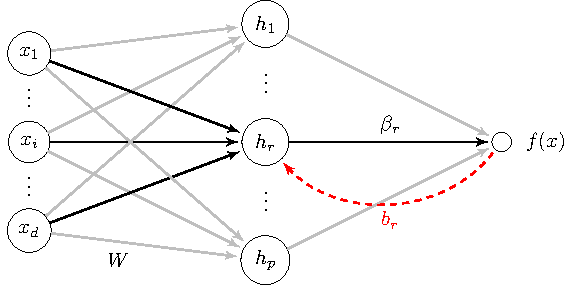
\includegraphics[width=.55\textwidth]{fig/fasketch}&\\[-1.8in]
    &
    \hskip-5pt
    \begin{minipage}{.47\textwidth}
    \begin{algorithm}[H]
    \centering
    \caption{Feedback Alignment}\label{algo:fa}
        \begin{algorithmic}[1]
            \Require Dataset $\{(x_i,y_i)\}_{i=1}^n$, step size $\eta$
            \State {\bf initialize} $W$, $\beta$ and $b$ as Gaussian
            \While{not converged}
                \State $\beta_r \gets \beta_r - \frac{\eta}{\sqrt p} \sum_{i=1}^n e_i \psi(w_r\transpose x_i)$
                \State $w_r \gets w_r - \frac{\eta}{\sqrt{p}} \sum_{i=1}^n e_i b_r\psi'(w_r\transpose x_i)x_i$
                \State for $r\in[p]$
            \EndWhile
        \end{algorithmic}
    \end{algorithm}%
    \end{minipage}
    \\[1.05in]

  \end{tabular}
\caption{Standard backpropagation updates the first layer weights for a hidden node $r$ with the second layer feedforward weight $\beta_r$. We study the procedure where the error is backpropagated instead using a fixed, random weight $b_r$.}
\label{fig:algo}
\end{figure*}


In the \textit{feedback alignment} procedure of \citep{lillicrap2016random},
when updating the weights $w_r$, the error signal is weighted not by the second layer feedforward weights $\beta$, but rather by a random set of weights $b\in\reals^p$ that are
fixed during the course of training. Equivalently, the gradients for the first layer are
replaced by the terms
\begin{align}\label{eqn:alignment-update}
  \widetilde{\frac{\partial\Loss}{\partial w_r}}   = \frac{1}{\sqrt{p}} \sum_{i=1}^n e_i b_r\psi'(w_r\transpose x_i)x_i.
\end{align}
Note, however, that this update rule does not correspond to the gradient with
respect to a modified loss function. The use of a random weight $b_r$ when updating
the first layer weights $w_r$ does not violate locality, and could conceivably be implemented by biological mechanisms; we refer to \cite{lillicrap2016random,bartunov,lillicrap2020backpropagation} for further discussion. A schematic of the relationship between the two algorithms is shown in Figure~\ref{fig:algo}.

We can now summarize the main results and contributions of this paper. Our first result shows that the error converges to zero when using random backpropagation weights.

\begin{itemize}
  \item Under Gaussian initialization of the parameters, if the model is sufficiently over-parameterized with $p\gg n$, then the error converges to zero linearly. Moreover, the parameters satisfy $\|w_r(t) - w_0(t) \| = \widetilde O\bigl(\frac{n}{\sqrt{p}}\bigr)$
    and $|\beta_r(t) - \beta_0(t) | = \widetilde O\bigl(\frac{n}{\sqrt{p}}\bigr)$.
\end{itemize}
The precise assumptions and statement of this result are given in \cref{thm:nonliner_conv}. The proof
shows that in the over-parameterized regime that the weights only change
by a small amount. While related to results for standard gradient descent,
new methods are required because the ``effective kernel'' is not positive semi-definite.

We next turn to the issue of alignment of the second layer parameters $\beta$ to the random backpropagation weights $b$. Such alignment was first observed in the original simulations of \cite{lillicrap2016random}. Intuitively, the possibility for alignment is seen in the fact that while the updates for $W$ use the error weighted by the random weights $b$, the updates for $\beta$ indirectly involve $W$, allowing for the possibility that dependence on $b$ will be introduced into $\beta$. However, the analysis is challenging. Our first result shows that, in fact, alignment will \textit{not} occur in the over-parameterized setting.
\begin{itemize}
\item The cosine of the angle between
these $p$-dimensional vectors $\beta$ and $b$ satisfies $ \cos\angle(b, \beta(t)) = O\big(\frac{n}{\sqrt p}\big)$.
\end{itemize}
In particular, while the error may converge, ``feedback alignment'' may be a bit of a misnomer for the algorithm, in general. However, we show that regularizing the parameters will cause the parameters $\beta$ to align with $b$. Our next result establishes this precisely in the linear case.
\begin{itemize}
\item Supposing that $\psi(u)=u$, then introducing a ridge penalty $\lambda(t) \|\beta\|^2$ where $\lambda(t) = \lambda$ for $t\leq T$ and $\lambda(t) = 0$ for $t > T$
on $\beta$  causes the parameters to align, with $\cos\angle(b, \beta(t)) \geq c > 0$ for sufficiently large $t$.
\end{itemize}
The technical conditions are given in \cref{thm:lin_align}.
Since $\beta(0)$ and $b$ are high dimensional Gaussian vectors, they are nearly orthogonal with high probability. The effect of regularization can be seen as shrinking the component of $\beta(0)$ in the parameters over time. Our simulations are consistent with this result, and also show alignment with a constant regularization $\lambda(t)\equiv \lambda$, for both linear and nonlinear activation functions. Finally, we complement this result by showing that convergence is preserved with regularization, for general activation functions. This is presented in \cref{thm:nonlinear_conv_reg}.

%%!TEX root=./main.tex
\section{Preliminaries}

We consider a two-layer neural network $f:\R^d \to \R$ with the hidden-layer width $p$, and for any input $x\in\Rd$, we have
\begin{align}\label{eqn:nonlinear-network}
    f(x) = \frac{1}{\sqrt p}\sum_{r=1}^p\beta_r\psi(w_r\transpose x)= \frac{1}{\sqrt p}\beta\transpose\psi(Wx),
\end{align}
where $\psi$ denotes the element-wise activation function, $W = (w_1,...,w_p)\transpose\in\Rpd$ and $\beta = (\beta_1,...,\beta_p)\transpose\in\Rp$ are the feed-forward weights for the first and the second layer.
Given $n$ input label pairs $\{(x_i,y_i)\}_{i=1}^n$, we hope to minimize the squared error loss
\begin{equation}
    \Loss(W,\beta) = \frac{1}{2}\sum_{i=1}^n \big(f(x_i)-y_i\big)^2.
\end{equation}
The gradient descent algorithm for minimizing the loss writes
\begin{align*}
    \beta_r(t+1) &= \beta_r(t)-\eta\frac{\partial\Loss}{\partial \beta_r}(W(t),\beta(t)), \\
    w_r(t+1) &= w_r(t)-\eta\frac{\partial\Loss}{\partial w_r}(W(t),\beta(t)), \quad r=1,\ldots,p.
\end{align*}
where $\eta>0$ is the step size, and we initialize $\beta(0)$ and $w_r(0)$ with standard Gaussian vectors. We also introduce the notations $u(t),e(t)\in \R^n$, where $u_i(t)$ is the network output on input $x_i$ at step $t$, $e_i(t) = u_i(t)-y$ is corresponding prediction error.

\paragraph{Backpropagation on two-layer network.}

Backpropagation has been the most commonly used scheme for computing the gradient of the network parameters. In particular, for two-layer network \eqref{eqn:nonlinear-network}, the gradients given by backpropagation are
\begin{equation*}
    \frac{\partial\Loss}{\partial \beta_r} = \frac{1}{\sqrt p}\sum_{i=1}^n e_i\psi(w_r\transpose x_i), \quad
    \frac{\partial\Loss}{\partial w_r} = \frac{1}{\sqrt p} \sum_{i=1}^n e_i \beta_r\psi'(w_r\transpose x_i)x_i.
\end{equation*}
However, such learning algorithm requires updating its weights with backpropagated error signals that consist of non-local information of weight parameters from top layers. More specifically, given an input $x_i$, the gradient of second-layer weights $\frac{\partial \Loss}{\partial \beta_r}$ contains only the local inputs $\psi(w_r x_i)$ and error signal $e_i = f(x_i) - y_i$, while the gradient of first-layer weights $\frac{\partial \Loss}{\partial w_r}$ requires not only the local input $x_i$, local output $w_r x_i$ but also the backpropagated error signal $e_i\beta_r$, which contains the information on the second-layer forward weights $\beta_r$. This appearance of $\beta_r$ is due to the chain rule between two adjacent layers and can be recognized as the backward weights in reverse propagation of error signals.
Consequently, backpropagation requires the forward weights between layers to be identical with the backward weights. However, from a biological perspective, this is a requirement on synaptic symmetry and is regarded as not biological plausible \citep{lillicrap2016random}. 

\paragraph{Feedback alignment on two-layer network.}

One of the alternative approaches proposed to improve the biological plausibility over backpropagation is \emph{Feedback Alignment}, which at the backpropagation stage replaces the forward weights at each layer by an independent fixed random backpropagation weights \citep{lillicrap2016random}. In particular, for the two-layer networks considered in this work, the second-layer weights $\beta$ is replaced by a fixed random backpropagation weights $b\in\Rp$ at backpropagation stage while the gradient update on $\beta$ remains the same, \ie,
\begin{align}\label{eqn:alignment-update}
    \dfa(w_r) = \frac{1}{\sqrt{p}} \sum_{i=1}^n e_i b_r\psi'(w_r\transpose x_i)x_i.
\end{align}
After the substitution, the feedback alignment update on $W$ no longer depends on $\beta$ directly and therefore bears no requirement on synaptic symmetry. Note that the path of $\beta(t)$ does not follow the one by gradient descent under standard backpropagation when considered jointly with the feedback alignment updates on $W(t)$. It is important to notice that the feedback alignment algorithm that we end up arriving at does not explicitly optimize on any particular loss function even though we motivate the algorithm from a loss function $\Loss$ and the corresponding gradient descent algorithm.
\cref{algo:fa} shows the feedback alignment algorithm on \eqref{eqn:nonlinear-network}.

%\begin{minipage}{\textwidth}
\begin{algorithm}[H]
\centering
\caption{Feedback Alignment on Two-Layer Networks}\label{algo:fa}
    \begin{algorithmic}[1]
        \Require activation $\psi$, dataset $\{(x_i,y_i)\}_{i=1}^n$, and step size $\eta$.
        \State {\bf initialize} $W(0)$, $\beta(0)$ and $b$ with standard Gaussian entries
        \While{not converge}
            \State $\beta_r(t+1) \gets \beta_r(t) - \frac{\eta}{\sqrt p} \sum_{i=1}^n e_i(t)\psi(w_r(t)\transpose x_i)$,
            \State $w_r(t+1) = w_r(t) - \frac{\eta}{\sqrt{p}} \sum_{i=1}^n e_i(t) b_r\psi'(w_r(t)\transpose x_i)x_i$, for $r=1,2,\ldots,p$.
        \EndWhile
    \end{algorithmic}    
\end{algorithm}%
%\end{minipage}



%!TEX root=./main.tex

\section{Convergence of Gradient Descent With Random Backpropagation Weights}

Due to the replacement of backward weights with the random backpropagation weights in feedback alignment algorithm, there is \emph{a priori} no guarantee that the algorithm will go downhill on the squared error loss $\Loss$. \citet{lillicrap2020backpropagation} study the convergence on two-layer linear networks under the continuous time setting. Through the analysis of a system of differential equations on network parameters, they show the convergence of the network to true linear target function under the assumption of infinite training data.
Among recent studies of over-parametrized networks under backpropagation, Neural Tangent Kernel (NTK) is heavily utilized to describe the evolution of the network during training process \citep{jacot2018neural}. For any neural network $f(x,\theta)$ with parameter $\theta$, the NTK is defined as
\begin{equation*}
	K_f(x,y) = \Big\langle \frac{\partial f (x,\theta)}{\partial \theta},\frac{\partial f (y,\theta)}{\partial \theta}\Big\rangle.
\end{equation*}
Given a dataset $\{(x_i,y_i)\}_{i=1}^n$, we can also consider its corresponding Gram matrix $K = (K_f(x_i,x_j))_{n\times n}$. \citet{jacot2018neural} show that in the infinite width limit, $K_f$ converges to a constant at initialization and does not drift away from initialization throughout training. Under the over-parameterized regime, if the Gram matrix $K$ is positive definite, then $K$ is going to stay close to the initialization during training and thus results in a linear convergence of the squared error loss \citep{du2018gradient,du2019gradient,gao2020model}.
% However, after replacing the feed-forward weights $\beta$ with a random backpropagation weights $b$, feedback alignment algorithm no longer follows a strict gradient descent on the squared error loss and the previous argument cannot be applied directly to our case. 
For the two-layer network $f(x, \theta)$ defined in \eqref{eqn:nonlinear-network} with $\theta = (\beta,W)$, the kernel $K_f$ can be written in two parts, $G_f$ and $H_f$, which correspond to $\beta$ and $W$ respectively:
\begin{equation}
K_f(x,y) = G_f(x, y) + H_f(x,y) \defeq \Big\langle \frac{\partial f (x,\theta)}{\partial \beta},\frac{\partial f (y,\theta)}{\partial \beta}\Big\rangle + \sum_{r=1}^p\Big\langle \frac{\partial f (x,\theta)}{\partial w_r},\frac{\partial f (y,\theta)}{\partial w_r}\Big\rangle.
\end{equation}
Under feedback alignment scheme with random backward weights $b$, $G_f$ remains the same as under backpropagation, while one of the gradient terms $\frac{\partial f}{\partial w_r}$ in $H_f$ is replaced by the feedback alignment update $\dfa(w_r)$ \eqref{eqn:alignment-update}, so $H_f$ it is no longer positive semi-definite and close to $0$ at initialization if the network is over-parameterized. However, if $G = (G_f(x_i,x_j))_{n\times n}$ is positive definite and $H = (H_f(x_i,x_j))_{n\times n}$ remains small during training, we are still able to show the loss $\Loss$ converging to zero exponentially fast. Specifically, we provide the following assumption and theorem.

\begin{assumption}\label{assump:G}
Define matrix $\overline{G} \in \R^{n\times n}$ with entries
$\overline{G}_{i,j} = \E_{w\sim \calN(0,I_p)}\psi(w\transpose x_i) \psi(w\transpose  x_j)$, we assume $\lambda_{\min}(\overline{G}) \geq \gamma$, where $\gamma$ is a positive constant.
\end{assumption}

\begin{theorem}\label{thm:nonliner_conv}
Let $W(0)$, $\beta(0)$ and $b$ have \iid standard Gaussian entries. Assume \textnormal{(1)} \cref{assump:G} holds, \textnormal{(2)} $\psi$ is smooth, $\psi$, $\psi'$ and $\psi''$ are bounded and \textnormal{(3)} $|y_i|$ and $\|x_i\|$ are bounded for all $i\in[n]$. Then there exists positive constants $c_1$, $c_2$, $C_1$ and $C_2$, such that for any $\delta\in(0,1)$, if $p \geq \max(C_1\frac{n^2}{\delta\gamma^2}, C_2\frac{n^4\log p}{\gamma^4})$, with probability at least $1-\delta$, we have
\begin{equation}\label{eq:conv}
    \|e(t+1)\| \leq (1-\frac{\eta\gamma}{4})\|e(t)\|
\end{equation}
and 
\begin{equation}
\label{eq:weights}
    \|w_r(t)-w_r(0)\| \leq c_1\frac{n\sqrt{\log p}}{\gamma\sqrt p}, \quad |\beta_r(t)-\beta_r(0)| \leq c_2\frac{n}{\gamma\sqrt p}
\end{equation}
for all $r=1,\ldots, p$ and $t>0$.
\end{theorem}

Notably, matrix $\overline{G}$ in \cref{assump:G} is the expectation of $G$ over random initialization and thus close to $\overline{G}$ due to concentration. To justify the assumption, we provide the following proposition, which states that \cref{assump:G} holds when $x_i$'s are drawn independently from Gaussian distribution. The proofs of \cref{thm:nonliner_conv,prop:positive-definiteness} are deferred to \cref{sec:appendix-convergence}.

\begin{proposition}\label{prop:positive-definiteness}
Suppose $x_1,...,x_n \overset{\iid}{\sim} \calN(0,I_d/d)$ and the activation function $\psi$ is sigmoid or tanh. If $d=\Omega(n)$, then \cref{assump:G} holds with high probability.
\end{proposition}





%!TEX root=./main.tex

\section{Alignment of Parameters to Random Backpropagation Weights}\label{sec:alignment}

The most prominent characteristic of feedback alignment algorithm is its phenomenon of alignment between the error signals back-propagated with forward weights and those with fixed random backward weights during training. Specifically, if we denote $h\in \R^p$ to be the hidden layer of the network, then we write $\dbp(h) \defeq \frac{\partial \Loss}{\partial h}$ to represent the error signals with respect to the hidden layer that are backpropagated with the feed-forward weights and $\dfa(h)$ as the error signals computed with fixed random backward weights.
\citet{lillicrap2016random} notice a decreasing angle between $\dbp(h)$ and $\dfa(h)$ during training, which suggests that feedback alignment algorithm can still carry gradient information back through layers even the signals are backpropagated through random weights.
In particular, the error signals $\dbp(h)$ and $\dfa(h)$ for the two-layer network \eqref{eqn:nonlinear-network} are given by 
\begin{equation}
    \dbp(h) = \frac{1}{\sqrt{p}}\beta\sum_{i=1}^ne_i \quad\text{and}\quad \dfa(h) = \frac{1}{\sqrt{p}}b\sum_{i=1}^ne_i,
\end{equation}
and the alignment can be characterized by the angle between $\beta(t)$ and $b$ during training. We formalize this concept of alignment by the following definition.
\begin{definition}\label{def:alignment}
    A series of vectors $\{\beta(t)\}_{t=0}^\infty$ align with a fixed vector $b$ if there exists a constant $c>0$ and time $T_c$ such that  $\cos\angle(b, \beta(t)) = \frac{\langle b, \beta(t)\rangle}{\|b\|\|\beta(t)\|} \geq c$ for all $t > T_c$.
\end{definition}

\subsection{Regularized Feedback Alignment}
Unfortunately, this alignment between $\beta(t)$ and $b$ is not guaranteed for over-parameterized networks and the loss \eqref{eqn:squared-loss}. To further illustrate our point, we control the cosine value of the angle by inequalities \eqref{eq:weights} from \cref{thm:nonliner_conv}, \ie,
\begin{equation}
    \Big|\cos\angle(b, \beta(t))\Big| \leq \frac{|\langle \frac{b}{\|b\|}, \beta(0)\rangle|+ \|\beta(t)- \beta(0)\|}{\|\beta(0)\|-\|\beta(t)-\beta(0)\|} = O\big(\frac{n}{\sqrt p}\big),
\end{equation}
which indicates that $\beta(t)$ and $b$ turn orthogonal as the network becomes wider. Intuitively, this can be understood as the parameters stay near their initializations during training when $p$ is large, where $\beta(0)$ and $b$ are almost orthogonal with each other. This motivates us to regularize the network parameters. Especially, we consider in this work the squared error loss with a $\ell_2$ regularization term on $\beta$:
\begin{equation}
\label{eqn:loss-with-reg}
\Loss(t, W, \beta) = \frac{1}{2}\sum_{i=1}^n\big(f(x_i)-y_i\big)^2 + \frac{1}{2}\lambda(t)\|\beta\|^2,
\end{equation}
where $\{\lambda(t)\}_{t=0}^\infty$ is a sequence of regularization rates, which defines a series of loss functions for different training steps $t$. The feedback alignment algorithm under the regularized loss are summarized in Algorithm \ref{algo:fa-reg}. Compared to \cref{algo:fa}, an extra contraction factor $1-\lambda(t)$ has been added in the update of $\beta(t)$, which doesn't affect the locality of the algorithm but helps the alignment by shrinking the component of $\beta(0)$ in $\beta(t)$.

%\begin{minipage}{\textwidth}
\begin{algorithm}[H]
\centering
\caption{Regularized Feedback Alignment on Two-Layer Networks}\label{algo:fa-reg}
    \begin{algorithmic}[1]
        \Require activation $\psi$, dataset $\{(x_i,y_i)\}_{i=1}^n$, and step size $\eta$, and regularization $\{\lambda(t)\}_t$.
        \State {\bf initialize} $W(0)$, $\beta(0)$ and $b$ with standard Gaussian entries
        \While{not converge}
            \State $\beta_r(t+1) \gets (1-\lambda(t))\beta_r(t) - \frac{\eta}{\sqrt p} \sum_{i=1}^n e_i(t)\psi(w_r(t)\transpose x_i)$ for $r\in[p]$
            \State $w_r(t+1) \gets w_r(t) - \frac{\eta}{\sqrt{p}} \sum_{i=1}^n e_i(t) b_r\psi'(w_r(t)\transpose x_i)x_i$ for $r\in[p]$
        \EndWhile
    \end{algorithmic}    
\end{algorithm}
%\end{minipage}

Following \cref{thm:nonliner_conv}, we also provide the error bound for regularized feedback alignment in \cref{thm:nonlinear_conv_reg}. Since regularization terms $\lambda(t)$ make additional contributions to the error $e(t)$ as well as to the kernel matrix $G$, an upper bound on $\sum_{t\geq 0}\lambda(t)$ is needed to ensure the positiveness of the minimal eigenvalue of $G$ during training, such that the error $e(t)$ can be controlled. In particular, if there is no regularization, \ie, $\lambda(t)=0$ for all $t\geq 0$, then we recover exponential convergence for the error $e(t)$ as in \cref{thm:nonliner_conv}. The proof of \cref{thm:nonlinear_conv_reg} is also deferred to \cref{sec:appendix-convergence}.
% didn't use G(t) since it is not defined before

\begin{theorem}
\label{thm:nonlinear_conv_reg}
Assume all the conditions from \cref{thm:nonliner_conv}. For \cref{algo:fa-reg}, assume $\sum_{t=0}^\infty \lambda(t) \leq  \tilde{S}_\lambda = \tilde{c}_{S}\frac{\gamma^2\sqrt{p}}{\eta n^2\sqrt{\log p}}$ for some constant $\tilde{c}_{S}$. Then there exists positive constants $C_1$ and $C_2$, such that for any $\delta\in(0,1)$, if $p \geq \max(C_1\frac{n^2}{\delta\gamma^2}, C_2\frac{n^4\log p}{\gamma^4})$, with probability at least $1-\delta$, we have for all $t\geq 0$
\begin{equation}
\label{eq:conv_reg}
    \|e(t+1)\| \leq \big(1-\frac{\eta\gamma}{4}-\eta\lambda(t)\big)\|e(t)\|+\lambda(t)\|y\|
\end{equation}
\end{theorem}



\subsection{Alignment Analysis on Linear Networks}
In this section, we focus on the theoretical analysis of alignment for linear networks, which is equivalent to setting the activation function $\psi$ into an identity map. The loss function can be written as
\begin{equation*}
    \Loss(t,W,\beta) = \frac{1}{2}\big\|\frac{1}{\sqrt{p}}XW\transpose\beta-y\big\|^2+\frac{\lambda(t)}{2}\|\beta\|^2,
\end{equation*}
where $X = (x_1,\ldots,x_n)\transpose$, and it is similar to the loss of ridge regression.
Before presenting our results on alignment, we first provide a linear version of \cref{thm:nonlinear_conv_reg} that adopts slightly different conditions.

\begin{theorem}
\label{thm:lin_conv}
Assume \textnormal{(1)}  $\|y\| = \Theta(\sqrt n)$, $\lambda_{\min}(XX\transpose)>\gamma$ and $\lambda_{\max}(XX\transpose)<M$ for some constants $M>\gamma>0$, and \textnormal{(2)} $\sum_{t=0}^\infty \lambda(t) \leq  S_\lambda = c_{S}\frac{\gamma\sqrt{\gamma p}}{\eta\sqrt{n}M}$ for some constant $c_{S}$.
For any $\delta\in(0,1)$, if $p = \Omega(\frac{Md\log(d/\delta)}{\gamma})$, the following inequality holds for all $t\geq 0$ with probability at least $1-\delta$
\begin{equation}
\label{eq:reg_error_bd}
\|e(t+1)\|\leq \big(1-\frac{\eta\gamma}{2}-\eta\lambda(t)\big)\|e(t)\| + \lambda(t)\|y\|.
\end{equation} 
\end{theorem}

We remark that, in the linear case, the kernel matrix $G$ reduces to the form $X W\transpose W X\transpose$ and its expectation $\overline{G}$ at initialization also reduces to $X X\transpose$, so \cref{assump:G} holds if $XX\transpose$ is positive definite, which is equivalent to $x_i$'s being linearly independent. The result of \cref{thm:nonlinear_conv_reg} can not be directly applied to linear case since we assume $\psi$ is bounded, which is true for sigmoid or tanh but not for identity map. This results in a slightly different order for $S_\lambda$ and an improved order for $p$.

Our results on alignment also rely on an isometric condition on $X$, which requires the minimum and the maximum eigenvalues of $XX\transpose$ to be close enough (\cf \cref{def:isom}). On the other hand, this condition is relatively mild and can be satisfied when $X$ has random Gaussian entries with a gentle dimensional constraint, as demonstrated by \cref{prop:isom}. Finally, we show in \cref{thm:lin_align} that under a simple regularization strategy where a constant regularization is adopted until a cutoff time $T$, regularized feedback alignment achieves alignment if $X$ satisfies the isometric condition.
{}
\begin{definition}[$(\gamma, \eps)$-Isometric]
\label{def:isom}
Given positive constant $\gamma$ and $\eps$, we say $X$ is $(\gamma, \eps)$-isometric if 
$\lambda_{\min}(XX\transpose)\geq\gamma$ and $\lambda_{\max}(XX\transpose)\leq(1+\eps)\gamma$.
\end{definition}

\begin{proposition}
\label{prop:isom}
Assume $X\in\R^{n\times d}$ has independent entries drawn from $N(0,1/d)$. For any $\eps \in (0,1/2)$ and $\delta \in (0,1)$, if $d=\Omega(\frac{1}{\eps}\log\frac{n}{\delta}+\frac{n}{\eps}\log \frac{1}{\eps})$, $X$ is $(1-\eps, 4\eps)$-isometric with probability $1-\delta$.
\end{proposition}

\begin{theorem}
\label{thm:lin_align}
Assume all conditions from \cref{thm:lin_conv} hold and $X$ is $(\gamma, \eps)$-isometric with a small constant $\eps$. Let the regularization weights
\begin{align*}
\lambda(t) = 
\begin{cases}
    \lambda, \quad t\leq T,\\
    0, \quad t > T,
\end{cases}
\end{align*}
with $\lambda=L\gamma$ and $T = \lfloor S_\lambda/\lambda\rfloor$ for some large constant $L$. Then, for any $\delta\in(0,1)$, if $p = \Omega(d\log(d/\delta))$, with probability at least $1-\delta$, regularized feedback alignment on linear network achieves alignment. Specifically, there exist a positive constant $c=c_\delta$ and time $T_c$, such that $\cos\angle(b, \beta(t))\geq c$ for all $t>T_c$.
\end{theorem}

We defer the proofs of \cref{prop:isom}, \cref{thm:lin_conv} and \cref{thm:lin_align} to \cref{sec:appendix-alignment}. In fact, we prove \cref{thm:lin_align} by directly computing $\beta(t)$ and the cosine of the angle. Although $b$ doesn't show up in the update of $\beta$, it could still propagate to $\beta$ through $W$. Since the amount of component of $b$ in $\beta(t)$ depends on the inner-product $\langle e(t), e(t')\rangle$ for all previous steps $t'\leq t$, the norm bound \eqref{eq:reg_error_bd} from \cref{thm:lin_conv} is insufficient so a more careful study on $e(t)$ is provided to accomplish the proof. We should point out that the constant $c$ in the lower bound is independent of the sample size $n$, input dimension $d$, network width $p$ and learning rate $\eta$. We also remark that the cutoff schedule of $\lambda(t)$ is just chosen for simplicity of the proof. For other schedules such as inverse-squared decay or exponential decay, one could also obtain the same alignment result as long as the summation of $\lambda(t)$ is less than $S_\lambda$.

\paragraph{Large sample scenario.} In \cref{thm:lin_conv,thm:lin_align}, we consider the case where sample size $n$ is less than input dimension $d$ so that the positive definiteness of $XX\transpose$ can be established. However, both results still hold for $n>d$. In fact, the squared error loss $\calL$ can be written as
\begin{equation*}
\sum_{i=1}^n\big(f(x_i)-y\big)^2 = \big\|\frac{1}{\sqrt{p}}XW\transpose\beta-y\big\|^2 = \big\|\frac{1}{\sqrt{p}}XW\transpose\beta-\bar{y}\big\|^2+ \|\bar{y}-y\|^2,
\end{equation*}
where $\bar{y}$ denotes the projection of $y$ onto the column space of $X$. Without loss of generality, we assume $y=\bar{y}$. As a result, $y$ and columns of $X$ are all in the same $d$-dimensional subspace of $\Rn$ and $XX\transpose$ is positive definite on this subspace as long as $X$ has full column rank. Consequently, we can either work on this subspace of $\Rn$ or project all the vectors onto $\Rd$, and the isometric condition are revised to only consider the $d$ nonzero eigenvalues of $XX\transpose$.
% with a left multiplication of $X\transpose$. (ganlin: actually U^T)



\section{Simulations}
\section{Discussion}

\clearpage
%\nocite{*} % Remove this line when needed
\bibliographystyle{apalike2}
\bibliography{feedback_alignment}

\clearpage
\section*{Checklist}

\begin{itemize}
    \item 
    Do the main claims made in the abstract and introduction accurately reflect the paper's contributions and scope?
    
    \answerYes{See abstract, Section 1, and Section 2 for the discussions on our main claims.}
    
    \item
    Have you read the ethics review guidelines and ensured that your paper conforms to them?
    
    \answerYes{}
    
    \item
    Did you discuss any potential negative societal impacts of your work?
    
    \answerTODO{}
    
    \item
    Did you describe the limitations of your work?
    
    \answerYes{See Section 6 for our discussion on the limitations.}
    
    \item
    Did you state the full set of assumptions of all theoretical results?
    
    \answerYes{See Section 3 and Section 4.}
    
    \item
    Did you include complete proofs of all theoretical results?
    
    \answerYes{Complete proofs are included in Appendix A and Appendix B.}
    
    \item
    Did you include the code, data, and instructions needed to reproduce the main experimental results (either in the supplemental material or as a URL)?
    
    \answerYes{They are included in the supplemental material.}
    
    \item
    Did you specify all the training details (e.g., data splits, hyperparameters, how they were chosen)?
    
    \answerYes{See Section 5 for the simulations.}
    
    \item
    Did you report error bars (e.g., with respect to the random seed after running experiments multiple times)?
    
    \answerYes{See Figure 2 and Figure 3.}
    
    \item
    Did you include the amount of compute and the type of resources used (e.g., type of GPUs, internal cluster, or cloud provider)?
    
    \answerYes{See Section 5.}
    
    \item
    If your work uses existing assets, did you cite the creators?
    
    \answerYes{See Section 5.}
    
    \item
    Did you mention the license of the assets?
    
    \answerYes{See Section 5.}
    
    \item
    Did you include any new assets either in the supplemental material or as a URL?
    
    \answerYes{They are included in the supplemental material.}
    
    \item
    Did you discuss whether and how consent was obtained from people whose data you're using/curating?
    
    \answerNA{Only external data used are MNIST data.}
    
    \item
    Did you discuss whether the data you are using/curating contains personally identifiable information or offensive content?
    
    \answerNA{Only external data used are MNIST data.}
\end{itemize}

\clearpage
\appendix
%!TEX root=./main.tex

\section{Convergence on Two-Layer Nonlinear Networks}\label{sec:appendix-convergence}
We consider the following neural network
\begin{equation}
f(x) = \frac{1}{\sqrt p}\sum_{r=1}^p \beta_r \psi(w_r\transpose x) = \frac{1}{\sqrt p}\beta\transpose \psi(Wx)
\end{equation}
where $\beta \in \R^p$, $W = (w_1,...,w_p)\transpose\in\R^{p\times d}$, and $\psi$ is activation function. Given data, the loss function is 
\begin{equation}
\Loss(W, \beta) = \frac{1}{2}\sum_{i=1}^n(f(x_i)-y_i)^2 = \frac{1}{2}\sum_{i=1}^n\Big(\frac{1}{\sqrt p}\beta\transpose \psi(Wx_i)-y\Big)^2
\end{equation}
The feedback alignment algorithm gives
\begin{equation}
\label{eq:updates}
\begin{aligned}
    W(t+1) &= W(t) - \eta\frac{1}{\sqrt p}\sum_{i=1}^nD_i(t)bx_i\transpose e_i(t) \\
    \beta(t+1) &= \beta(t)- \eta \frac{1}{\sqrt p}\sum_{i=1}^n \psi(W(t)x_i)e_i(t)
\end{aligned}
\end{equation}
where $D_i(t) = \text{diag}(\psi'(W(t)x_i))$ and $e_i(t) = \frac{1}{\sqrt p}\beta(t)\transpose \psi(W(t)x_i)-y_i$. We also denote $u(t)\in\R^n$ with $u_i(t) = \frac{1}{\sqrt p}\beta(t)\transpose \psi(W(t)x_i)$, the network prediction on $x_i$ at time $t$. To make the proof clear, we use $c$, $C$ as the global constants whose values may vary from line to line.

\subsection{Concentration Results}

\begin{lemma}[Lemma A.7 in \citealp{gao2020model}]\label{lma:G}
Assume $x_1,...,x_n \overset{\iid}{\sim} \calN(0,I_d/d)$. We define  matrix $\widetilde{G}\in \R^{n\times n}$ with entries
\begin{equation*}
    \widetilde{G}_{i,j} = |\E\psi'(Z)|^2 \frac{x_i\transpose x_j}{\|x_i\|\|x_j\|} + (\E|\psi(Z)|^2-|\E\psi'(Z)|^2)\I\{i=j\}
\end{equation*}
where $Z\sim \calN(0,1)$. If $d = \Omega(\log n)$, then with high probability, we have
\begin{equation*}
\|\overline{G}-\widetilde{G}\|^2 \lesssim \frac{\log n}{d} + \frac{n^2}{d^2}
\end{equation*}
\end{lemma}


\begin{proof}[Proof of \cref{prop:positive-definiteness}]
In fact, if $\psi$ is sigmoid or tanh, for a standard Gaussian random variable $Z$, we have
\begin{equation*}
    \gamma\defeq \frac{1}{2}(\E|\psi(Z)|^2-|\E\psi'(Z)|^2) >0.
\end{equation*}
From \cref{lma:G}, we know that with high probability $\lambda_{\min}(\overline{G}) \geq \lambda_{\min}(\widetilde{G})-\|\overline{G}-\widetilde{G}\|\geq 2\gamma - C(\sqrt{\frac{\log n}{d}} + \frac{n}{d}) \geq \gamma$.
\end{proof}

\begin{lemma}
\label{lma:inqs}
Assume $W(0)$, $\beta(0)$ and $b$ have \iid standard Gaussian entries. Given $\delta\in(0,1)$, if $p=\Omega(n/\delta)$, then with probability $1-\delta$
\begin{equation}\label{eq:sumb_bd}
    \frac{1}{p}\sum_{r=1}^p|b_r| \leq c,
\end{equation}
\begin{equation}\label{eq:sumbbet_bd}
    \frac{1}{p}\sum_{r=1}^p|b_r\beta_r(0)| \leq c,
\end{equation}
\begin{equation}\label{eq:e0_bd}
    \|e(0)\| \leq c\sqrt n,
\end{equation}
\begin{equation}\label{eq:maxb_bd}
    \max_{r\in[p]}|b_r|\leq 2\sqrt{\log p}.
\end{equation}
\end{lemma}
\begin{proof}
We will show each inequality holds with probability at least $1-\frac{\delta}{4}$, then by a union bound, all of them hold with probability at least $1-\frac{\delta}{4}$. Since $\Var(\frac{1}{p}\sum_{r=1}^p|b_r|)\leq \frac{\Var(|b_0|)}{p}$, by Chebyshev's inequality, we have 
\begin{equation*}
    \prob(\frac{1}{p}\sum_{r=1}^p|b_r| > \E(b_1) + 1) \leq \frac{\Var(|b_1|)}{p} \leq \delta/4
\end{equation*} 
if $p\geq 4\Var(|b_1|)/\delta$, which gives \eqref{eq:sumb_bd}. The proof for \eqref{eq:sumbbet_bd} is similar since $\Var(\frac{1}{p}\sum_{r=1}^p|b_r\beta_r(0)|)=O(1/p)$. To prove \eqref{eq:e0_bd}, since $|y_i|$ and $\|x_i\|$ are bounded, it suffices to show $|u_i(0)|\leq c$ for all $i\in [n]$. Actually, by independence, we have
\begin{equation*}
    \Var(u_i(0)) = \Var \Big(\frac{1}{p}\sum_{r=1}^p \beta_r(0)\psi(w_r(0)\transpose x_i)\Big) = \frac{1}{p}\Var\Big(\beta_1(0)\psi(w_1(0)\transpose x_i)\Big) = O(1/p).
\end{equation*}
By Chebyshev's inequality, we have for each $i\in [n]$
\begin{equation*}
    \prob(|u_i(0)|> c) \leq \frac{\Var(u_i(0))}{c^2} \leq \frac{\delta}{4n}
\end{equation*}
where we require $p=\Omega(n/\delta)$. With a union bound argument, we could show \eqref{eq:e0_bd}. Finally, \eqref{eq:maxb_bd} is followed from standard Gaussian tail bound and union bound argument, \ie,
\begin{equation*}
    \prob(\max_{r\in[p]}|b_r| > 2\sqrt{\log p}) \leq \sum_{r\in [p]}\prob(|b_r| > 2\sqrt{\log p}) \leq 2pe^{-2\log p} = \frac{2}{p} \leq \frac{\delta}{4}
\end{equation*}
\end{proof}

\begin{lemma}
\label{lma:GH}
Under the conditions of \cref{thm:nonliner_conv}, we define matrix $G(0),H(0)\in\R^{n\times n}$ with entries
\begin{equation}
\label{eq:def_G0}
G_{ij}(0) = \frac{1}{p}\psi(W(0)x_i)\transpose \psi(W(0)x_j) = \frac{1}{p}\sum_{r=1}^p\psi(w_r(0)\transpose x_i)\psi(w_r(0)\transpose x_j) 
\end{equation}
and 
\begin{equation}
\label{eq:def_H0}
H_{ij}(0) = \frac{x_i\transpose x_j}{p}\beta(0)\transpose D_i(0)D_j(0)b = \frac{1}{p}\sum_{r=1}^p\beta_r(0)b_r\psi'(w_r(0)\transpose x_i)\psi'(w_r(0)\transpose x_j).
\end{equation}
For any $\delta \in (0,1)$, if $p=\Omega(\frac{n^2}{\delta\gamma^2})$, then with probability at least $1-\delta$, we have $\lambda_{\min}(G(0))\geq \frac{3}{4}\gamma$ and $\|H(0)\|\leq \frac{\gamma}{4}$.
\end{lemma}
\begin{proof}
By independence and boundedness of $\psi$ and $\psi'$, we have $\Var(G_{ij}(0)) = O(1/p)$ and $\Var(H_{ij}(0)) = O(1/p)$. Since $\E(G(0))=\overline{G}$, we have
\begin{equation*}
\E\|G(0)-\overline{G}\|^2 \leq \E\|G(0)-\overline{G}\|^2_F = O(\frac{n^2}{p})
\end{equation*}
by Markov's inequality, when $p=\Omega(\frac{n^2}{\delta\gamma^2})$
\begin{equation*}
    \prob(\|G(0)-\overline{G}\|>\frac{\gamma}{4})\leq O(\frac{n^2}{p\gamma^2})\leq\frac{\delta}{2}
\end{equation*}
Similarly we have $\prob(\|H(0)\|>\frac{\gamma}{4})\leq\frac{\delta}{2}$, since $\E(H(0))=0$. Then with probability at least $1-\delta$, $\lambda_{\min}(G(0)) \geq \lambda_{\min}(\overline{G}) -\gamma/4 \geq \frac{3}{4}\gamma$, and $\|H(0)\|\leq \gamma/4$.
\end{proof}

\subsection{Proof of Theorem \ref{thm:nonliner_conv}}

\begin{lemma}
\label{lma:weights}
Assume all the inequalities from \cref{lma:inqs} holds. Under the conditions of \cref{thm:nonliner_conv}, if the error bound \eqref{eq:conv} holds for all $t=1,2,...,t'-1$, then the bounds \eqref{eq:weights} hold for all $t\leq t'$.
\end{lemma}

\begin{proof}
From the feedback alignment updates \eqref{eq:updates}, we have for all $t\leq T$.
\begin{equation*}
\begin{aligned}
    |\beta_r(t)-\beta_r(0)| &\leq \frac{\eta}{\sqrt p}\sum_{s=0}^{t-1}\sum_{i=1}^n |\psi(w_r(t)x_i)e_i(t)| \\
    &\leq c\frac{\eta}{\sqrt p}\sum_{s=0}^{t-1}\sum_{i=1}^n |e_i(t)| \\
    &\leq c\frac{\eta\sqrt n}{\sqrt p}\sum_{s=0}^{t-1} \|e(t)\| \\
    &\leq c\frac{\eta\sqrt n}{\sqrt p}\sum_{s=0}^{t-1}  (1-\frac{\gamma\eta}{4})^t\|e(0)\|  \\
    &\leq c\frac{\sqrt n}{\gamma\sqrt p}\|e(0)\| \\
    &\leq c\frac{n}{\gamma\sqrt p}
\end{aligned}
\end{equation*}
where we use $\psi$ is bounded and \eqref{eq:e0_bd}. We also have
\begin{equation*}
\begin{aligned}
    \|w_r(t)-w_r(0)\| &\leq \frac{\eta}{\sqrt p}\sum_{s=0}^{t-1}\sum_{i=1}^n \|\psi'(w_r(t)\transpose x_i)b_rx_i e_i(t)\| \\
    & \leq c\frac{\eta}{\sqrt p}\sum_{s=0}^{t-1}\sum_{i=1}^n |b_r| |e_i(t)| \\
    & \leq c|b_r|\frac{\eta\sqrt n}{\sqrt p}\sum_{s=0}^{t-1} \|e(t)\| \\
    & \leq c|b_r|\frac{\sqrt n}{\gamma\sqrt p}\|e(0)\| \\
    & \leq c\frac{n\sqrt{\log p}}{\gamma\sqrt p}
\end{aligned}
\end{equation*}
where we use $\psi'$ is bounded, \eqref{eq:e0_bd} and \eqref{eq:maxb_bd}.
\end{proof}

\begin{lemma}
\label{lma:induction}
Assume all the inequalities from \cref{lma:inqs} holds. Under the conditions of \cref{thm:nonliner_conv}, if the bound for weights difference \eqref{eq:weights} holds for all $t\leq t'$ and error bound \eqref{eq:conv} holds for all $t\leq t'-1$, then \eqref{eq:conv} holds for $t=t'$.
\end{lemma}
\begin{proof}
We start with analyzing the error $e(t)$
\begin{equation*}
\begin{aligned}
    e_i(t+1) 
    &= \frac{1}{\sqrt p}\beta(t+1)\transpose\psi(W(t+1)x_i) - y_i \\
    &= \frac{1}{\sqrt p}\beta(t+1)\transpose(\psi(W(t+1)x_i)-\psi(W(t)x_i))+ \frac{1}{\sqrt p}(\beta(t+1)-\beta(t))\transpose \psi(W(t)x_i) \\
    & \quad + \frac{1}{\sqrt p}\beta(t)\transpose \psi(W(t)x_i) - y_i \\
    &=e_i(t) - \frac{\eta}{p}\beta(t+1)\transpose D_i(t)\sum_{j=1}^nD_j(t)b x_j\transpose x_i e_j(t)  - \frac{\eta}{p}\sum_{j=1}^n\psi(W(t)x_j)\transpose\psi(W(t)x_i)e_j(t) \\
    & \quad + v_i(t) \\
    & = e_i(t)-\eta\sum_{j=1}^n\big(H_{ij}(t)+G_{ij}(t)\big)e_j(t) + v_i(t)
\end{aligned}
\end{equation*}
where
\begin{equation*}
\begin{aligned}
G_{ij}(t) &= \frac{1}{p}\psi(W(t)x_j)\transpose\psi(W(t)x_i) \\
H_{ij}(t) &= \frac{x_i\transpose x_j}{p}\beta(t+1)\transpose D_i(t)D_j(t)b
\end{aligned}
\end{equation*}
and $v_i(t)$ is the residual term from the Taylor's expansion
\begin{equation*}
    v_i(t) = \frac{1}{2\sqrt p}\sum_{r=1}^p\beta_r(t+1)|(w_r(t+1)-w_r(t))\transpose x_i|^2\psi''(\xi_{ri}(t))
\end{equation*}
with $\xi_{ri}(t)$ between $w_r(t)\transpose x_i$ and $w_r(t+1)\transpose x_i$. We can also rewrite the above iteration in a vector form
\begin{equation}\label{eq:et_iter}
     e(t+1) = e(t) - \eta(G(t)+H(t))e(t) + v(t)
\end{equation} 
Now for $t=t'-1$, we try to show that both $G(t)$ and $H(t)$ are close to their initialization. Notice that
\begin{equation*}
\begin{aligned}
    |G_{ij}(t) - G_{ij}(0)| 
    & = \frac{1}{p}\Big|\psi(W(t)x_j)\transpose\psi(W(t)x_i) -\psi(W(t)x_j)\transpose\psi(W(t)x_i)\Big| \\
    & \leq \frac{1}{p} \sum_{r=1}^p |\psi(w_r(t)\transpose x_j)||\psi(w_r(t)\transpose x_i)-\psi(w_r(0)\transpose x_i)| \\
    &\quad + \frac{1}{p} \sum_{r=1}^p |\psi(w_r(0)\transpose x_i)||\psi(w_r(t)\transpose x_j)-\psi(w_r(0)\transpose x_j)| \\
    &\leq c \frac{1}{p} \sum_{r=1}^p|w_r(t)\transpose x_i-w_r(0)\transpose x_i| + \frac{1}{p} \sum_{r=1}^p|w_r(t)\transpose x_j-w_r(0)\transpose x_j| \\
    &\leq c_0 \frac{n\sqrt{\log p}}{\gamma\sqrt p} (\|x_i\|+\|x_j\|)
\end{aligned}
\end{equation*}
where the second inequality is due to the boundedness of $\psi$ and $\psi'$, the last inequality is by \eqref{eq:weights}, then we have
\begin{equation}\label{eq:bound_Gt}
    \|G(t)-G(0)\| \leq \max_{j \in [n]}\sum_{i=1}^n|G_{ij}(t) - G_{ij}(0)| \leq c_0 \frac{n^2\sqrt{\log p}}{\gamma\sqrt p}
\end{equation}
For matrix $H(t)$, similarly we have
\begin{equation*}
\begin{aligned}
    |H_{ij}(t)-H_{ij}(0)|
    &\leq \frac{|x_i\transpose x_j|}{p}\Big|\beta(t+1)\transpose D_i(t)D_j(t)b - \beta(0)\transpose D_i(0)D_j(0)b\Big| \\
    &\leq \frac{\|x_i\|\|x_j\|}{p}\sum_{r=1}^p \Big|b_r\beta_r(t+1)\psi'(w_r(t)\transpose x_i)\psi'(w_r(t)\transpose x_j)\\
    &\quad -b_r\beta_r(0)\psi'(w_r(0)\transpose x_i)\psi'(w_r(0)\transpose x_j)\Big| \\
    &\leq \frac{|\|x_i\|\|x_j\||}{p}\sum_{r=1}^p\Big(|b_r||\beta_r(t+1)-\beta_r(0)| |\psi'(w_r(t)\transpose x_i)\psi'(w_r(t)\transpose x_j)|\\
    & \quad +|b_r||\beta_r(0)| |\psi'(w_r(t)\transpose x_i)-\psi'(w_r(0)\transpose x_i)| |\psi'(w_r(t)\transpose x_j)|\\
    & \quad +|b_r||\beta_r(0)| |\psi'(w_r(0)\transpose x_i)| |\psi'(w_r(t)\transpose x_j)-\psi'(w_r(0)\transpose x_j)| \Big)\\
    &\leq c\frac{\|x_i\|\|x_j\|}{p}\sum_{r=1}^p\Big(|b_r|\frac{n}{\gamma\sqrt p} + |b_r||\beta_r(0)|\frac{n\sqrt{\log p}}{\gamma\sqrt p} (\|x_i\|+\|x_j\|)\Big) \\
    &\leq c_1 \frac{n}{\gamma\sqrt p} + c_2\frac{n\sqrt{\log p}}{\gamma\sqrt p}.
\end{aligned}
\end{equation*}
It follows
\begin{equation}\label{eq:bound_Ht}
    \|H(t)-H(0)\| \leq \max_{j \in [n]}\sum_{i=1}^n|H_{ij}(t) - H_{ij}(0)| \leq c_1 \frac{n^2}{\gamma\sqrt p} + c_2\frac{n^2\sqrt{\log p}}{\gamma\sqrt p}
\end{equation}
Next, we bound the residual term $v_i(t)$. Since $\psi''$ is bounded, we have
\begin{equation*}
\begin{aligned}
    |v_i(t)|
    &\leq c\frac{1}{\sqrt p}\sum_{r=1}^p|\beta_r(t+1)|\|w_r(t+1)-w_r(t)\|^2 \\
    &\leq c\frac{1}{\sqrt p}\frac{\eta^2}{p}\sum_{r=1}^p|\beta_r(t+1)|\Big(\sum_{i=1}^n\|\psi'(w_r(t)\transpose x_i)b_rx_ie_i(t)\|\Big)^2 \\
    &\leq c\frac{1}{\sqrt p}\frac{\eta^2}{p}\sum_{r=1}^p|\beta_r(t+1)||b_r|^2\Big(\sum_{i=1}^n|e_i(t)|\Big)^2 \\
    &\leq c\frac{\eta^2n}{\sqrt p}\|e(t)\|^2 \\
    &\leq c_3\frac{\eta^2n\sqrt n}{\sqrt p}\|e(t)\|
\end{aligned}
\end{equation*}
It gives the bound
\begin{equation}\label{eq:bound_vt}
    \|v(t)\| =\Big(\sum_{i=1}^n|v_i(t)|^2\Big)^{1/2} \leq c_3\frac{\eta^2n^2}{\sqrt p}\|e(t)\|
\end{equation}
Combining \cref{eq:et_iter,eq:bound_Gt,eq:bound_Ht,eq:bound_vt}, we have
\begin{equation*}
\begin{aligned}
\|e(t+1)\| 
&\leq \|I_n-\eta (G(t)+H(t))\|\|e(t)\|+\|v(t)\| \\
&\leq \Big(\|I_n-\eta G(0)\|+\eta\|G(t)-G(0)\|+\eta\|H(0)\| \\
&\quad +\eta\|H(t)-H(0)\|\Big)\|e(t)\| + \|v(t)\| \\
&\leq \Big( 1-\frac{3\eta\gamma}{4}+c_0\frac{\eta n^2\sqrt{\log p}}{\gamma\sqrt p}+\frac{\eta\gamma}{4}+c_1\frac{\eta n^2}{\gamma\sqrt p} + c_2\frac{\eta n^2\sqrt{\log p}}{\gamma\sqrt p}+c_3\frac{\eta^2n\sqrt n}{\sqrt p}\Big)\|e(t)\|  \\
&\leq(1-\frac{\eta\gamma}{4})\|e(t)\|
\end{aligned}
\end{equation*}
where we use the \cref{lma:GH} and $p=\Omega(\frac{n^4\log p}{\gamma^4})$.
\end{proof}

\begin{proof}[Proof of \cref{thm:nonliner_conv}]
We prove the inequality \eqref{eq:conv} by induction. Suppose \eqref{eq:conv} and \eqref{eq:weights} hold for all $t=1,2,...,t'-1$, by \cref{lma:weights} and \cref{lma:induction} we know \eqref{eq:conv} and \eqref{eq:weights} hold for $t=t'$, which completes the proof.
\end{proof}

\subsection{Proof of Theorem \ref{thm:nonlinear_conv_reg}}

\begin{lemma}
\label{lma:weights_reg}
Assume all the inequalities from \cref{lma:inqs} holds. Under the conditions of \cref{thm:nonlinear_conv_reg}, if the error bound \eqref{eq:conv_reg} holds for all $t=1,2,...,t'-1$, then 
\begin{equation}
\label{eq:weights_reg}
\begin{aligned}
    \|w_r(t)-w_r(0)\| &\leq c_1\frac{n\sqrt{\log p}}{\gamma\sqrt p}(1+\eta \tilde{S}_\lambda),\\
    |\beta_r(t)-\beta_r(0)| &\leq c_2\frac{n}{\gamma\sqrt p}(1+\eta \tilde{S}_\lambda)
\end{aligned}
\end{equation}
hold for all $t\leq t'$, where $c_1$, $c_2$ are constants.
\end{lemma}

\begin{proof}
For any $k\leq t'-1$, we apply \eqref{eq:conv_reg} repeatedly on the right hand side of itself to get
\begin{equation*}
    \|e(k)\|\leq \prod_{i=0}^{k-1}\Big(1-\frac{\eta\gamma}{4}-\eta\lambda(i)\Big)\|e(0)\| + \sum_{i=0}^{k-1}\eta\lambda(i)\prod_{i<j<k}\Big(1-\frac{\eta\gamma}{4}-\eta\lambda(j)\Big)\|y\|
\end{equation*}
For $t\leq t'-1$, we take the sum over $k=0,..,t$ on both sides of above inequality 
\begin{equation*}
\begin{aligned}
    \sum_{k=0}^{t}\|e(k)\|
    &\leq \sum_{k=0}^{t}\prod_{i=0}^{k-1}\Big(1-\frac{\eta\gamma}{4}-\eta\lambda(i)\Big)\|e(0)\|  + \sum_{k=0}^{t}\sum_{i=0}^{k-1}\eta\lambda(i)\prod_{i<j<k}\Big(1-\frac{\eta\gamma}{4}-\eta\lambda(j)\Big)\|y\| \\
    &\leq \sum_{k=0}^{t}\Big(1-\frac{\eta\gamma}{4}\Big)^{k-1}\|e(0)\|+ \sum_{k=0}^{t}\sum_{i=0}^{k-1}\eta\lambda(i)\Big(1-\frac{\eta\gamma}{4}\Big)^{k-i-1}\|y\| \\
    &\leq \sum_{k=0}^{t}\Big(1-\frac{\eta\gamma}{4}\Big)^{k-1}\|e(0)\| + \eta\|y\|\sum_{k=0}^{t-1}\lambda(i)\sum_{k=i+1}^T\Big(1-\frac{\eta\gamma}{4}\Big)^{k-i-1} \\
    &\leq \frac{4}{\eta\gamma}\|e(0)\|+ \frac{4}{\gamma}\tilde{S}_\lambda\|y\| \\
    &\leq \frac{c\sqrt n}{\gamma}(\frac{1}{\eta}+\tilde{S}_\lambda)
\end{aligned}
\end{equation*} 
where we use $\|e(0)\|=O(\sqrt n)$ and $\|y\|=O(\sqrt n)$. Then for all $t\leq t'$, we have
\begin{equation*}
\begin{aligned}
    |\beta_r(t)-\beta_r(0)| &\leq \frac{\eta}{\sqrt p}\sum_{s=0}^{t-1}\sum_{i=1}^n |\psi(w_r(t)x_i)e_i(t)| \\
    &\leq c\frac{\eta}{\sqrt p}\sum_{s=0}^{t-1}\sum_{i=1}^n |e_i(t)| \\
    &\leq c\frac{\eta\sqrt n}{\sqrt p}\sum_{s=0}^{t-1} \|e(t)\| \\
    &\leq c\frac{\eta\sqrt n}{\sqrt p}\frac{\sqrt n}{\gamma}(\frac{1}{\eta}+\tilde{S}_\lambda)  \\
    &\leq c\frac{n}{\gamma\sqrt p} (1+\eta \tilde{S}_\lambda)
\end{aligned}
\end{equation*}
where we use $\psi$ is bounded and \eqref{eq:e0_bd}. We also have
\begin{equation*}
\begin{aligned}
    \|w_r(t)-w_r(0)\| &\leq \frac{\eta}{\sqrt p}\sum_{s=0}^{t-1}\sum_{i=1}^n \|\psi'(w_r(t)\transpose x_i)b_rx_i e_i(t)\| \\
    & \leq c\frac{\eta}{\sqrt p}\sum_{s=0}^{t-1}\sum_{i=1}^n |b_r| |e_i(t)| \\
    & \leq c|b_r|\frac{\eta\sqrt n}{\sqrt p}\sum_{s=0}^{t-1} \|e(t)\| \\
    & \leq c|b_r|\frac{\eta\sqrt n}{\sqrt p}\frac{\sqrt n}{\gamma}(\frac{1}{\eta}+\tilde{S}_\lambda) \\
    & \leq c\frac{n\sqrt{\log p}}{\gamma\sqrt p} (1+\eta \tilde{S}_\lambda)
\end{aligned}
\end{equation*}
where we use $\psi'$ is bounded, \eqref{eq:e0_bd} and \eqref{eq:maxb_bd}.
\end{proof}


\begin{lemma}
\label{lma:induction_reg}
Assume all the inequalities from \cref{lma:inqs} holds. Under the conditions of \cref{thm:nonlinear_conv_reg}, if the bound for weights difference \eqref{eq:weights_reg} holds for all $t\leq t'$ and error bound \eqref{eq:conv_reg} holds for all $t\leq t'-1$, then \eqref{eq:conv_reg} holds for $t=t'$.
\end{lemma}
\begin{proof}
We start with analyzing the error $e(t)$
\begin{equation*}
\begin{aligned}
    e_i(t+1) 
    &= \frac{1}{\sqrt p}\beta(t+1)\transpose\psi(W(t+1)x_i) - y_i \\
    &= \frac{1}{\sqrt p}\beta(t+1)\transpose(\psi(W(t+1)x_i)-\psi(W(t)x_i))+ \frac{1}{\sqrt p}(\beta(t+1)-(1-\eta\lambda(t))\beta(t))\transpose \psi(W(t)x_i) \\
    & \quad + (1-\eta\lambda(t))\Big(\frac{1}{\sqrt p}\beta(t)\transpose \psi(W(t)x_i) - y_i\Big) - \eta\lambda(t)y \\
    &=(1-\eta\lambda(t))e_i(t) - \frac{\eta}{p}\beta(t+1)\transpose D_i(t)\sum_{j=1}^nD_j(t)b x_j\transpose x_i e_j(t)  - \frac{\eta}{p}\sum_{j=1}^n\psi(W(t)x_j)\transpose\psi(W(t)x_i)e_j(t) - \eta\lambda(t)y\\
    & \quad + v_i(t) \\
    & = (1-\eta\lambda(t))e_i(t)-\eta\sum_{j=1}^n\big(H_{ij}(t)+G_{ij}(t)\big)e_j(t) + v_i(t) - \eta\lambda(t)y
\end{aligned}
\end{equation*}
where
\begin{equation*}
\begin{aligned}
G_{ij}(t) &= \frac{1}{p}\psi(W(t)x_j)\transpose\psi(W(t)x_i) \\
H_{ij}(t) &= \frac{x_i\transpose x_j}{p}\beta(t+1)\transpose D_i(t)D_j(t)b
\end{aligned}
\end{equation*}
and $v_i(t)$ is the residual term from the Taylor's expansion
\begin{equation*}
    v_i(t) = \frac{1}{2\sqrt p}\sum_{r=1}^p\beta_r(t+1)|(w_r(t+1)-w_r(t))\transpose x_i|^2\psi''(\xi_{ri}(t))
\end{equation*}
with $\xi_{ri}(t)$ between $w_r(t)\transpose x_i$ and $w_r(t+1)\transpose x_i$. We can also rewrite the above iteration in a vector form
\begin{equation}\label{eq:et_iter_reg}
     e(t+1) = (1-\lambda(t))e(t) - \eta(G(t)+H(t))e(t) + v(t) -\eta\lambda(t)y
\end{equation} 
Now for $t=t'-1$, we try to show that both $G(t)$ and $H(t)$ are close to their initialization. Similar to the argument in \cref{lma:induction}, we can obtain the following bound
\begin{equation}\label{eq:bound_Gt_reg}
    \|G(t)-G(0)\| \leq c_1 \frac{n^2\sqrt{\log p}}{\gamma\sqrt p}(1+\eta \tilde{S}_\lambda)
\end{equation}

\begin{equation}\label{eq:bound_Ht_reg}
    \|H(t)-H(0)\| \leq c_2\frac{n^2\sqrt{\log p}}{\gamma\sqrt p}(1+\eta \tilde{S}_\lambda)
\end{equation}
\begin{equation}\label{eq:bound_vt_reg}
    \|v(t)\| \leq c_3\frac{\eta^2n^2}{\sqrt p}\|e(t)\|
\end{equation}
Combining \cref{eq:et_iter_reg,eq:bound_Gt_reg,eq:bound_Ht_reg,eq:bound_vt_reg}, we have
\begin{equation*}
\begin{aligned}
\|e(t+1)\| 
&\leq \|(1-\eta\lambda(t))I_n-\eta (G(t)+H(t))\|\|e(t)\|+\|v(t)\| \\
&\leq \Big(\|(1-\eta\lambda(t))I_n-\eta G(0)\|+\eta\|G(t)-G(0)\|+\eta\|H(0)\| \\
&\quad +\eta\|H(t)-H(0)\|\Big)\|e(t)\| + \|v(t)\| \\
&\leq \Big( 1-\eta\lambda(t)-\frac{3\eta\gamma}{4}+(c_1+ c_2)\frac{\eta n^2\sqrt{\log p}}{\gamma\sqrt p}(1+\eta \tilde{S}_\lambda)+c_3\frac{\eta^2n\sqrt n}{\sqrt p}\Big)\|e(t)\|  \\
&\leq(1-\eta\lambda(t)-\frac{\eta\gamma}{4})\|e(t)\|
\end{aligned}
\end{equation*}
where we use the \cref{lma:GH}, $p=\Omega(\frac{n^4\log p}{\gamma^4})$ and $\tilde{S}_\lambda = O(\frac{\gamma^2\sqrt{p}}{\eta n^2\sqrt{\log p}})$.
\end{proof}

\begin{proof}[Proof of \cref{thm:nonlinear_conv_reg}]
We prove the inequality \eqref{eq:conv_reg} by induction. Suppose \eqref{eq:conv_reg} holds for all $t=1,2,...,t'-1$, by \cref{lma:weights_reg} and \cref{lma:induction_reg} we know \eqref{eq:conv_reg} holds for $t=t'$, which completes the proof.
\end{proof}
\section{Alignment on Two-Layer Linear Networks}\label{sec:appendix-alignment}

Now we assume $\psi = \mathbbm{1}$, or $f$ is a linear network. The loss function with regularization at time $t$ is
\begin{equation}
\label{eq:reg_loss}
\Loss(t, W, \beta) = \frac{1}{2}\big\|\frac{1}{\sqrt p}XW\transpose\beta-y\big\|^2 + \frac{1}{2}\lambda(t)\|\beta\|^2
\end{equation}
The regularized feedback alignment algorithm gives
\begin{equation}
\label{eq:reg_alg}
\begin{aligned}
    W(t+1) &= W(t) - \eta\frac{1}{\sqrt p}b e(t)\transpose X\\
    \beta(t+1) &= (1-\eta\lambda(t))\beta(t)- \frac{\eta}{\sqrt p} W(t)X\transpose e(t)
\end{aligned}
\end{equation}
where $e(t)=\frac{1}{\sqrt p}XW(t)\transpose \beta(t)-y$ is the error vector at time t.


\begin{lemma}
\label{lma:one_step_update}
Suppose the network is trained with regularized feedback alignment algorithm \eqref{eq:reg_alg}, then the prediction error $e(t)$ follows the iteration update
\begin{equation}
\label{eq:err_update}
\begin{aligned}
    e(t+1) = \bigg[(1-\eta\lambda(t))I_d - \frac{\eta}{p}XW(0)\transpose W(0)X\transpose -\eta\Big(J_1(t)+J_2(t)+J_3(t)\Big)\bigg]e(t) -\eta\lambda(t)y
\end{aligned}
\end{equation}
where
\begin{equation*}
\begin{aligned}
&J_1(t) = \frac{1}{p}b\transpose\beta(0)\prod_{i=0}^{t}(1-\eta\lambda(i))XX\transpose \\
&J_2(t) = -\frac{\eta}{p}\Big(\bar{v}\transpose X\transpose \hat{s}(t) XX\transpose+ XX\transpose s(t-1)\bar{v}\transpose X\transpose + X \bar{v}s(t-1)\transpose XX\transpose\Big) \\
&J_3(t) = \frac{\eta^2}{p^2}\|b\|^2\Big(\hat{S}(t)XX\transpose + XX\transpose s(t-1)s(t-1)\transpose XX\transpose)
\end{aligned}
\end{equation*}
and
\begin{equation*}
\begin{aligned}
&\bar{v} = \frac{1}{\sqrt p}W(0)\transpose b \\
&s(t) = \sum_{i=0}^{t}e(i) \\
&\hat{s}(t) = \sum_{i=0}^{t}\prod_{i<k\leq t}(1-\eta\lambda(k)) e(i) \\
&\hat{S}(t) = \sum_{i=0}^{t}\prod_{i<k\leq t}(1-\eta\lambda(k))e(i)\transpose XX\transpose \sum_{j=0}^{i-1}e(j).
\end{aligned}
\end{equation*}
\end{lemma}

\begin{proof}
We first write $W(t)$ in terms of $W(0)$ and $e(i)$, $i\in[t]$
\begin{equation}
\label{eq:Wt}
    W(t) = W(0) -\frac{\eta}{\sqrt p} b\sum_{i=0}^{t-1}e(i)\transpose X = W(0) -\frac{\eta}{\sqrt p} bs(t-1)\transpose X.
\end{equation}
Similarly, for $\beta(t)$ we have
\begin{equation}
\label{eq:betat}
\begin{aligned}
    \beta(t) &=\prod_{i=0}^{t-1}(1-\eta\lambda(i))\beta(0)-\frac{\eta}{\sqrt p}\sum_{i=0}^{t-1}\prod_{i<k<t}(1-\eta\lambda(k))W(i)X\transpose e(i) \\
    &=\prod_{i=0}^{t-1}(1-\eta\lambda(i))\beta(0)-\frac{\eta}{\sqrt p}\sum_{i=0}^{t-1}\prod_{i<k<t}(1-\eta\lambda(k))\Big(W(0) -\frac{\eta}{\sqrt p} b\sum_{j=0}^{i-1}e(j)\transpose X\Big)X\transpose e(i) \\
    &=\prod_{i=0}^{t-1}(1-\eta\lambda(i))\beta(0)-\frac{\eta}{\sqrt p}\sum_{i=0}^{t-1}\prod_{i<k<t}(1-\eta\lambda(k))W(0)X\transpose e(i)\\
    &\quad + \frac{\eta^2}{p}b\sum_{i=0}^{t-1}\prod_{i<k<t}(1-\eta\lambda(k))e(i)\transpose XX\transpose \sum_{j=0}^{i-1}e(j) \\
    &=\prod_{i=0}^{t-1}(1-\eta\lambda(i))\beta(0) -\frac{\eta}{\sqrt p}W(0)X\transpose \hat{s}(t-1) +\frac{\eta^2}{p}b \hat{S}(t-1).
\end{aligned}
\end{equation}
We now study how error $e(t)$ changes after one step of update
\begin{equation*}
\begin{aligned}
    e(t+1) &= \frac{1}{\sqrt p}XW(t+1)\transpose \beta(t+1)-y \\
    &= \frac{1}{\sqrt p}X(W(t+1)-W(t)\transpose \beta(t+1)+ \frac{1}{\sqrt p}XW(t)\transpose (\beta(t+1)-(1-\eta\lambda(t))\beta(t)) \\
    &\quad +(1-\eta\lambda(t))\Big(\frac{1}{\sqrt p}XW(t)\transpose \beta(t)-y\Big) -\eta\lambda(t)y\\
    &=(1-\eta\lambda(t))e(t) - \frac{\eta}{p}b\transpose\beta(t+1)XX\transpose e(t)  - \frac{\eta}{p}XW(t)\transpose W(t)X\transpose e(t) - \eta\lambda(t)y
\end{aligned}
\end{equation*}
By plugging \eqref{eq:Wt} and \eqref{eq:betat} into above equation, we have
\begin{equation*}
\begin{aligned}
    e(t+1) &= (1-\eta\lambda(t))e(t) \\
    &\quad-\frac{\eta}{p}b\transpose\bigg[ \prod_{i=0}^{t}(1-\eta\lambda(i))\beta(0) -\frac{\eta}{\sqrt p}W(0)X\transpose \hat{s}(t) +\frac{\eta^2}{p}b \hat{S}(t)\bigg]XX\transpose e(t) \\
    &\quad - \frac{\eta}{p}X\bigg[W(0) -\frac{\eta}{\sqrt p}bs(t-1)\transpose X\bigg]\transpose \bigg[W(0) -\frac{\eta}{\sqrt p}bs(t-1)\transpose X\bigg]X\transpose e(t)\\
    &\quad - \eta\lambda(t)y
\end{aligned}
\end{equation*}
After expanding the brackets and rearranging the items, we can obtain \eqref{eq:err_update}.
\end{proof}

\begin{lemma}
\label{lma:ineqs_2}
Given $\delta\in(0,1)$ and $\epsilon>0$ , if $p=\Omega(\frac{1}{\epsilon}\log\frac{d}{\delta}+\frac{d}{\epsilon}\log\frac{1}{\epsilon})$, the following inequalities hold with probability at least $1-\delta$
\begin{equation}
\label{eq:bbeta_sqrtp}
\frac{|b\transpose\beta(0)|}{\sqrt p}\leq c\sqrt{\log\frac{1}{\delta}}
\end{equation}
\begin{equation}
\label{eq:bW_sqrtp}
\frac{\|b\transpose W(0)\|}{\sqrt p}\leq c\sqrt{d\log\frac{d}{\delta}}
\end{equation}
\begin{equation}
\label{eq:b_norm}
\Big|\frac{\|b\|^2}{p}-1\Big| \leq  \frac{c}{\sqrt p}\sqrt {\log \frac{1}{\delta}}
\end{equation}
\begin{equation}
\label{eq:ww_p}
\Big\|\frac{1}{p}W(0)\transpose W(0) - I_d \Big\|\leq \epsilon
\end{equation}
where $c$ is a constant.
\end{lemma}

\begin{proof}
\eqref{eq:bbeta_sqrtp} is derived from \cref{lem:inner-product-tail}. \eqref{eq:bW_sqrtp} is by \eqref{eq:bbeta_sqrtp} and a union bound argument. \eqref{eq:b_norm} is by \cref{lem:chi-squared-tail}. \eqref{eq:ww_p} is by \cref{cor:RIP}
\end{proof}

\begin{proof}[Proof of Theorem \ref{thm:lin_conv}]
We show \eqref{eq:reg_error_bd} by induction. Assume \eqref{eq:reg_error_bd} holds for all $t=0,1,...,t'$, we will show it hold for $t=t'+1$. For any $k\leq t'$, we apply \eqref{eq:reg_error_bd} repeatedly on the right hand side of itself to get
\begin{equation*}
    \|e(k)\|\leq \prod_{i=0}^{k-1}\Big(1-\frac{\eta\gamma}{2}-\eta\lambda(i)\Big)\|e(0)\| + \sum_{i=0}^{k-1}\eta\lambda(i)\prod_{i<j<k}\Big(1-\frac{\eta\gamma}{2}-\eta\lambda(j)\Big)\|y\|
\end{equation*}
For $t\leq t'$, we take the sum over $k=0,..,t$ on both sides of above inequality
\begin{equation*}
\begin{aligned}
    \sum_{k=0}^{t}\|e(k)\|
    &\leq \sum_{k=0}^{t}\prod_{i=0}^{k-1}\Big(1-\frac{\eta\gamma}{2}-\eta\lambda(i)\Big)\|e(0)\|  + \sum_{k=0}^{t}\sum_{i=0}^{k-1}\eta\lambda(i)\prod_{i<j<k}\Big(1-\frac{\eta\gamma}{2}-\eta\lambda(j)\Big)\|y\| \\
    &\leq \sum_{k=0}^{t}\Big(1-\frac{\eta\gamma}{2}\Big)^{k-1}\|e(0)\|+ \sum_{k=0}^{t}\sum_{i=0}^{k-1}\eta\lambda(i)\Big(1-\frac{\eta\gamma}{2}\Big)^{k-i-1}\|y\| \\
    &\leq \sum_{k=0}^{t}\Big(1-\frac{\eta\gamma}{2}\Big)^{k-1}\|e(0)\| + \eta\|y\|\sum_{k=0}^{t-1}\lambda(i)\sum_{k=i+1}^T\Big(1-\frac{\eta\gamma}{2}\Big)^{k-i-1} \\
    &\leq \frac{2}{\eta\gamma}\|e(0)\|+ \frac{2}{\gamma}S_\lambda\|y\| \\
    &\leq \frac{c\sqrt n}{\gamma}(\frac{1}{\eta}+S_\lambda)
\end{aligned}
\end{equation*}
where we use $\|e(0)\|=O(\sqrt n)$ and $\|y\|=O(\sqrt n)$. With this bound and the inequalities from \cref{lma:ineqs_2}, we can bound the norms of $J_1(t)$, $J_2(t)$ and $J_3(t)$ from \cref{lma:one_step_update}. It follows that
\begin{equation}
\label{eq:J1_bd}
\|J_1(t)\| \leq \frac{1}{p}|b\transpose\beta(0)|\|XX\transpose\|\leq c\frac{M\sqrt{\log \delta^{-1}}}{\sqrt p}\leq \frac{\gamma}{16},
\end{equation}
\begin{equation}
\label{eq:J2_bd}
\|J_2(t)\| \leq \frac{\eta}{p}\|X\| \|XX\transpose\|\|\bar{v}\|(2\|s(t-1)\|+\|\hat{s}(t)\|)\leq c\frac{\eta}{p}M^{3/2}\sqrt{d\log\frac{d}{\delta}}\frac{\sqrt n}{\gamma}(\frac{1}{\eta}+S_\lambda)\leq \frac{\gamma}{16}
\end{equation}
and
\begin{equation}
\label{eq:J3_bd}
\|J_3(t)\| \leq \frac{\eta^2}{p^2}\|b\|^2(\|XX\transpose\| |\hat{S}(t)|+\|XX\transpose\|^2 \|s(t-1)\|^2) \leq c\frac{\eta^2}{p}M^2 \frac{n}{\gamma^2}(\frac{1}{\eta}+S_\lambda)^2\leq \frac{\gamma}{16}
\end{equation}
hold for all $t\leq t'$ if $p = \Omega(\frac{Md\log(d/\delta)}{\gamma})$ and $S_\lambda = O(\frac{\gamma\sqrt{\gamma p}}{\eta\sqrt{n}M})$. Furthermore, since $\|\frac{1}{p}W(0)W(0)\transpose-I_d\|\leq \epsilon_0$ with high probability when $p=\Omega(d)$, we have
\begin{equation}
\label{eq:xwwx_bd}
\begin{aligned}
\|\frac{1}{p}XW(0)\transpose W(0)X\transpose-\gamma I_d\|
&\leq \|\frac{1}{p}XW(0)\transpose W(0)X\transpose-XX\transpose\| + \|XX\transpose-\gamma I_d\|  \\
&\leq (1+\epsilon)\epsilon_0\gamma+\epsilon\gamma \leq \frac{\gamma}{16}
\end{aligned}
\end{equation}
Therefore, combining \eqref{eq:J1_bd}, \eqref{eq:J2_bd}, \eqref{eq:J3_bd} and \eqref{eq:err_update}, we have
\begin{equation*}
\begin{aligned}
       \|e(t'+1)\|
       &\leq \Big(1-\eta\lambda(t')-\eta\gamma\Big) \|e(t')\| + \eta\Big\|\frac{\eta}{p}XW(0)\transpose W(0)X\transpose-\gamma I_d\Big\|\|e(t')\|\\
       &\quad + \eta(\|J_1(t')\|+\|J_2(t')\|+\|J_3(t')\|)\|e(t')\| + \eta\lambda(t')\|y\| \\
       &\leq \Big(1-\eta\lambda(t')-\eta\gamma\Big)\|e(t')\| + \frac{1}{16}\eta\gamma\|e(t')\|+ \frac{3}{16}\eta\gamma\|e(t')\|  + \eta\lambda(t')\|y\| \\
       &\leq\Big(1-\eta\lambda(t')-\frac{\eta\gamma}{2}\Big)\|e(t')\| +  \eta\lambda(t')\|y\|
\end{aligned}
\end{equation*}
which completes the proof.
\end{proof}


\begin{proof}[Proof of Proposition \ref{prop:isom}]
By \cref{cor:RIP}, if $d=\Omega(\frac{1}{\epsilon}\log\frac{n}{\delta}+\frac{n}{\epsilon}\log \frac{1}{\epsilon})$, we have
\begin{equation*}
\|XX\transpose - I_n\|\leq \epsilon
\end{equation*}
It follows that $\lambda_{\min}(XX\transpose)\geq 1-\epsilon$ and $\lambda_{\max}(XX\transpose)\leq 1+\epsilon \leq (1+4\epsilon)(1-\epsilon)$ for $\epsilon <1/2$.
\end{proof}


\begin{lemma}
\label{lma:suf_cond}
Recall from \cref{lma:one_step_update} that
\begin{equation*}
\beta(t)=\prod_{i=0}^{t-1}(1-\eta\lambda(i))\beta(0) -\frac{\eta}{\sqrt p}W(0)X\transpose \hat{s}(t-1) +\frac{\eta^2}{p}b \hat{S}(t-1)
\end{equation*}
with $\hat{s}(t) = \sum_{i=0}^{t}\prod_{i<k\leq t}(1-\eta\lambda(k)) e(i)$ and $\hat{S}(t) = \sum_{i=0}^{t}\prod_{i<k\leq t}(1-\eta\lambda(k))e(i)\transpose XX\transpose \sum_{j=0}^{i-1}e(j)$. Under the conditions of Theorem \ref{thm:lin_align}, if $t>C_1\frac{\log (p/\eta)}{\eta\lambda}$ and $\hat{S}(t)\geq \max(C_2\frac{\sqrt{p\gamma}}{\eta}\|\hat{s}(t)\|,1)$ for some positive constants $C_1$ and $C_2$, then $\cos\angle(b, \beta(t)) \geq c$ for some constant $c=c_\delta$.
\end{lemma}
\begin{proof}
We compute the cosine of the angle between $\beta(t)$ and $b$. With probability $1-\delta$,
\begin{equation*}
\begin{aligned}
    \cos\angle(b, \beta(t))
    &= \frac{b\transpose \beta(t)}{\|b\|\|\beta(t)\|}= \frac{\frac{b}{\|b\|}\transpose \beta(t)}{\|\beta(t)\|}\\
    &\geq \frac{\frac{\eta^2}{p}\|b\|\hat{S}(t-1) - (1-\eta\lambda)^t\|\beta(0)\| - \frac{\eta}{\sqrt p}\|\frac{b}{\|b\|}\transpose W(0)\|\|X\|\|\hat{s}(t-1)\|}{\frac{\eta^2}{p}\|b\|\hat{S}(t-1)+(1-\eta\lambda)^t\|\beta(0)\| + \frac{\eta}{\sqrt p}\|W(0)\|\|X\|\|\hat{s}(t-1)\|} \\
    &\geq \frac{c'_1\frac{\eta^2}{\sqrt p}\hat{S}(t-1) - c'_2\sqrt p(1-\eta\lambda)^t- c'_3\eta\sqrt{\frac{d\gamma}{p}}\|\hat{s}(t-1)\|}{c'_1\frac{\eta^2}{\sqrt p}\hat{S}(t-1) + c'_2\sqrt p(1-\eta\lambda)^t+ c'_4\eta\sqrt{\gamma}\|\hat{s}(t-1)\|}
\end{aligned}
\end{equation*}
where we use \eqref{eq:b_norm}, \eqref{eq:ww_p} and the tail bound for standard Gaussian vectors, and $c'_i$, $i\in[4]$ are constant that only depends on $\delta$. Notice that if $t=\Omega(\frac{\log (p/\eta)}{\eta\lambda})$, we have $c'_2\sqrt p(1-\eta\lambda)^t = O(\frac{\eta^2}{\sqrt p})$. It follows that $\cos\angle(b, \beta(t)) \geq c$ if $\hat{S}(t-1)=\Omega(\frac{\sqrt{p\gamma}}{\eta}\|\hat{s}(t-1)\|+1)$.
\end{proof}

\begin{lemma}
\label{lma:decomp_1}
We take the orthogonal decomposition $e(t) = a(t)\bar{y}+\xi(t)$, where $\bar{y}=-y/\|y\|$ and $\xi(t)\perp y$. Under the conditions of Theorem \ref{thm:lin_align}, there exists constant $C_\tau>0$ such that for any $t\in[\tau,T]$ with $\tau=\frac{C_\tau}{\eta\lambda}$, we have
\begin{equation}
\label{eq:at_lbd}
a(t)\geq \frac{\lambda - \gamma}{\lambda+\gamma}\|y\|
\end{equation}
and
\begin{equation}
\label{eq:xit_ubd}
\|\xi(t)\|\leq \frac{\gamma}{\lambda+\gamma}\|y\|
\end{equation}
\end{lemma}

\begin{proof}
By Theorem \ref{thm:lin_conv}, we have for all $t\leq T$, $\|e(t)\|\leq(1-\eta\lambda-\eta\gamma/2)\|e(t)\|+\eta\lambda\|y\|$. By rearranging the terms, we have
\begin{equation*}
    \|e(t+1)\| -\frac{\lambda }{\lambda - \gamma/2}\|y\| \leq (1-\eta\lambda-\frac{\eta\gamma}{2})\Big(\|e(t)\| -\frac{\lambda }{\lambda - \gamma/2}\|y\|\Big)
\end{equation*}
or
\begin{equation*}
\|e(t)\| -\frac{\lambda }{\lambda - \gamma/2}\|y\|\leq (1-\eta\lambda-\frac{\eta\gamma}{2})^t \Big(\|e_0\|- \frac{\lambda }{\lambda - \gamma/2}\|y\|\Big) \leq (1-\eta\lambda)^t(\|e_0\|+\|y\|)
\end{equation*}
Notice that $\|y\|$ and $\|e(0)\|$ are in the same order, so when $t\in [\tau_1,T]$ with $\tau_1 = \frac{c_1}{\eta\lambda}$ and some constant $c_1$, we have
\begin{equation}
\label{eq:et_y_bd}
\|e(t)\|\leq \frac{\lambda+\gamma/2}{\lambda-\gamma/2} \|y\|
\end{equation}
In order to get a lower bound of $a(t)$, we multiply $\bar{y}\transpose$ on both sides of \eqref{eq:err_update}. It follows that for $t\in [\tau_1,T]$
\begin{equation*}
\begin{aligned}
a(t+1)
&\geq \bar{y}\transpose\Big(1-\eta\lambda-\eta\gamma\Big)e(t) - \eta\|\frac{1}{p}XW(0)\transpose W(0)X\transpose-\gamma I_d\|\|e(t)\|\\
&\quad-\eta(\|J_1(t)\|+\|J_2(t)\|+\|J_3(t)\|)\|e(t)\| +\eta\lambda\|y\|  \\
&\geq (1-\eta\lambda-\eta\gamma)a(t)- \frac{1}{4}\eta\gamma \|e(t)\| +\eta\lambda\|y\| \\
&\geq (1-\eta\lambda-\eta\gamma)a(t)+\frac{1}{2}\eta\gamma\|y\|
\end{aligned}
\end{equation*}
In the second inequality, we use the bounds \eqref{eq:J1_bd}, \eqref{eq:J2_bd}, \eqref{eq:J3_bd} and \eqref{eq:xwwx_bd}. The last inequality is by \eqref{eq:et_y_bd} and $\lambda\geq 3\gamma$. Follow the similar derivation, we have
\begin{equation*}
a(t) -\frac{\lambda - \gamma/2}{\lambda +\gamma}\|y\|\geq (1-\eta\lambda-\eta\gamma)^{t-\tau_1} \Big(a(\tau_1)- \frac{\lambda - \gamma/2}{\lambda +\gamma}\|y\|\Big) \geq -(1-\eta\lambda)^{t-\tau_1}(\|e(\tau_1)\|+\|y\|)
\end{equation*}
The bound \eqref{eq:at_lbd} holds when $t\in [\tau_1+\tau_2,T]$ with $\tau_2 = \frac{c_2}{\eta\lambda}$ and some constant $c_2$. Then we multiply $\frac{\xi(t+1)\transpose}{\|\xi(t+1)\|}$ on both sides of \eqref{eq:err_update}. It gives that for $t\in [\tau_1,T]$
\begin{equation*}
\begin{aligned}
\|\xi(t+1)\|
&\leq \frac{\xi(t+1)\transpose}{\|\xi(t+1)\|}\Big(1-\eta\lambda-\eta\gamma\Big)e(t) + \eta\|\frac{1}{p}XW(0)\transpose W(0)X\transpose-\gamma I_d\|\|e(t)\|\\
&\quad+\eta(\|J_1(t)\|+\|J_2(t)\|+\|J_3(t)\|)\|e(t)\| +\eta\lambda\|y\|  \\
&\leq (1-\eta\lambda-\eta\gamma)\|\xi(t)\|+ \frac{\eta\gamma}{4}\|e(t)\| \\
&\leq (1-\eta\lambda-\eta\gamma)\|\xi(t)\|+ \frac{\eta\gamma}{2}\eta\gamma\|y\|
\end{aligned}
\end{equation*}
The first inequality is by $\xi(t+1)\transpose y =0$ and in the second inequality we use $\xi(t+1)\transpose e(t) = \xi(t+1)\transpose\xi(t) \leq \|\xi(t+1)\|\|\xi(t)\|$. It follows that
\begin{equation*}
\|\xi(t)\|-\frac{\gamma/2}{\lambda+\gamma}\|y\|\leq (1-\eta\lambda-\eta\gamma)^{t-\tau_1}\Big(\|\xi(0)\|-\frac{\gamma/2}{\lambda+\gamma}\|y\|\Big)\leq (1-\eta\lambda)^{t-\tau_1}(\|e(\tau_1)\|+\|y\|)
\end{equation*}
The bound \eqref{eq:xit_ubd} holds when $t\in [\tau_1+\tau_3,T]$ with $\tau_3 = \frac{c_3}{\eta\lambda}$ and some constant $c_3$. Finally, the bound \eqref{eq:at_lbd} and \eqref{eq:xit_ubd} hold when $t\in[\tau,T]$ with $\tau = \tau_1 + \max(\tau_2,\tau_3)$.
\end{proof}


\begin{lemma}
\label{lma:ST_sT}
Under the conditions of Theorem \ref{thm:lin_align}. Given $T = \lfloor \frac{S_\lambda}{\lambda} \rfloor = C_T\frac{\sqrt{p}}{\eta\sqrt{n\gamma}}$. We have $\hat{S}(T) \geq \tilde{c}\frac{\sqrt {p\gamma}}{\eta}\|\hat{s}(T)\|$, where $C_T$ and $\tilde{c}$ are positive constants.
\end{lemma}
\begin{proof}
Notice that
\begin{equation*}
    e(i)\transpose XX\transpose e(j) \geq \gamma e(i)\transpose e(j) - \|e(i)\|\|e(j)\|\|XX\transpose-\gamma I\| \geq \gamma e(i)\transpose e(j) - \epsilon\gamma\|e(i)\|\|e(j)\|
\end{equation*}
For $i\in[T/2,T]$ and $\tau$ defined in \cref{lma:decomp_1}, we have
\begin{equation}
\label{eq:eXXe}
\begin{aligned}
    e(i)\transpose XX\transpose \sum_{j<i}e(j)
    &= e(i)\transpose XX\transpose \sum_{\tau\leq j<i}e(j) + e(i)\transpose XX\transpose \sum_{j<\tau}e(j) \\
    &\geq \sum_{\tau\leq j<i}\Big(\gamma e(i)\transpose e(j) - \epsilon\gamma\|e(i)\|\|e(j)\|\Big) - 2\gamma \sum_{j<\tau}\|e(i)\|\|e(j)\| \\
    &\geq \sum_{\tau\leq j<i}\gamma\Big(a(i)a(j) - \|\xi(i)\|\|\xi(j)\| - \epsilon\|e(i)\|\|e(j)\|\Big) - 2c\tau\gamma \|y\|^2 \\
    &\geq (i-\tau)\gamma\Big[\Big(\frac{\lambda-\gamma}{\lambda+\gamma}\Big)^2\|y\|^2-\Big(\frac{\gamma}{\lambda+\gamma}\Big)^2\|y\|^2-\epsilon\Big(\frac{\lambda+\gamma/2}{\lambda-\gamma/2}\Big)^2\|y\|^2- \frac{2c\tau}{i-\tau}\|y\|^2\Big] \\
    &\geq \frac{T}{8}\gamma\|y\|^2 = \frac{C_T}{8}\frac{\sqrt{p}}{\eta\sqrt{n\gamma}}\gamma\|y\|^2 \\
    &\geq c\frac{\sqrt{p\gamma}}{\eta}\|y\|
\end{aligned}
\end{equation}
The second inequality is by orthogonal decomposition of $e(i)$ and $\|e(i)\|\leq c\|y\|$ given by \eqref{eq:reg_error_bd}. The third inequality is by \eqref{eq:at_lbd}, \eqref{eq:xit_ubd} and \eqref{eq:et_y_bd} from \cref{lma:decomp_1}. The fourth inequality is by $\lambda=\Omega(\gamma)$, $i-\tau \geq T/4$ and $\tau/(i-\tau)$ is small ($p=\Omega(n)$). The last inequality is by $\|y\|=\Theta(\sqrt n)$. Therefore,
\begin{equation*}
\begin{aligned}
    \hat{S}(T) &= \sum_{i=0}^T(1-\eta\lambda)^{T-i}e(i)\transpose XX\transpose \sum_{j<i}e(j) \\
    &= \sum_{i=T/2}^T(1-\eta\lambda)^{T-i}e(i)\transpose XX\transpose \sum_{j<i}e(j) + (1-\eta\lambda)^{T/2}\sum_{i=0}^{T/2}(1-\eta\lambda)^{T/2-i}e(i)\transpose XX\transpose \sum_{j<i}e(j) \\
    &\geq \sum_{i=T/2}^T(1-\eta\lambda)^{T-i}c\frac{\sqrt{p\gamma}}{\eta}\|y\| + (1-\eta\lambda)^{T/2}\sum_{i=0}^{T/2}(1-\eta\lambda)^{T/2-i}c'T\gamma\|y\|^2 \\
    &\geq \frac{c}{2}\frac{\sqrt{p\gamma}}{\eta}\frac{\|y\|}{\eta\lambda} -(1-\eta\lambda)^{T/2}\frac{c'T\gamma\|y\|^2}{\eta\lambda} \\
    &\geq \frac{c}{4}\frac{\sqrt{p\gamma}}{\eta}\frac{\|y\|}{\eta\lambda}
\end{aligned}
\end{equation*}
where the last inequality is by $(1-\eta\lambda)^{T/2}\ll 1$ when $p=\Omega(n)$. On the other hand,
\begin{equation*}
\begin{aligned}
\|\hat{s}(T)\|
&\leq \sum_{i=0}^T(1-\eta\lambda)^{T-i}\|e(i)\|\leq \frac{c}{\eta\lambda}\|y\|
\end{aligned}
\end{equation*}
Combining the above inequalities gives the proof.
\end{proof}

\begin{proof}[Proof of Theorem \ref{thm:lin_align}]
First, notice that $\lambda(t)=0$ when $t>T$. By Theorem \ref{thm:lin_conv} we have the prediction error converges to 0 exponentially fast, or $\|e(t+1)\|\leq (1-\eta\gamma/2)\|e(t)\|$. It follows $\hat{S}(t)\to \hat{S}(\infty)$ and $\hat{s}(t)\to \hat{s}(\infty)$ as $t\to\infty$. By \cref{lma:suf_cond}, we know it suffices to show $\hat{S}(\infty)\geq C\frac{\sqrt{p\gamma}}{\eta}\|\hat{s}(\infty)\|$ with some constant $C$. Since
\begin{equation*}
\hat{S}(\infty) = \sum_{i=0}^\infty(1-\eta\lambda)^{(T-i)_+}e(i)\transpose XX\transpose \sum_{j<i} e(j) = \hat{S}(T)+ \sum_{i>T}e(i)\transpose XX\transpose \sum_{j<i}e(j)
\end{equation*}
and
\begin{equation*}
\hat{s}(\infty) = \sum_{i=0}^\infty(1-\eta\lambda)^{(T-i)_+}e(i)= \hat{s}(T)+ \sum_{i>T}e(i),
\end{equation*}
by \cref{lma:ST_sT}, it suffices to show
\begin{equation}
\label{eq:exxe_e_bd}
    \sum_{i>T}e(i)\transpose XX\transpose \sum_{j<i}e(j) \geq C\frac{\sqrt{p\gamma}}{\eta}\sum_{i>T}\|e(i)\|
\end{equation}
We write $g = XX\transpose \sum_{j<T}e(j)$. It holds that
\begin{equation}
\label{eq:g_lbd}
\begin{aligned}
\|g\| &\geq \lambda_{\min}(XX\transpose) \Big[\Big\|\sum_{\tau\geq j<T}e(j)\Big\|-\sum_{j<\tau}\|e(j)\|\Big] \\
&\geq\lambda_{\min}(XX\transpose) \Big[\sum_{\tau\geq j<T}a(j)-\sum_{j<\tau}\|e(j)\|\Big] \\
&\geq \gamma\Big[(T-\tau)\Big(\frac{\lambda-\gamma}{\lambda+\gamma}\Big)\|y\| - \tau c\|y\|\Big]
\end{aligned}
\end{equation}
and
\begin{equation}
\label{eq:g_ubd}
\begin{aligned}
\|g\| &\leq \|XX\transpose\| \Big(\sum_{j<\tau}\|e(j)\| + \sum_{\tau\geq j<T}\|e(j)\|\Big) \\
&\leq (1+\epsilon)\gamma\Big[\tau c\|y\|+ (T-\tau)\Big(\frac{\lambda+\gamma/2}{\lambda-\gamma/2}\Big)\|y\|\Big]
\end{aligned}
\end{equation}
where we use the bounds \eqref{eq:at_lbd} and \eqref{eq:et_y_bd} from \cref{lma:decomp_1}. We further denote $\alpha(t) = \bar{g}\transpose e(t)$ where $\bar{g} = g/\|g\|$. Following the same calculation in \eqref{eq:eXXe}, we have
\begin{equation*}
\begin{aligned}
    g\transpose e(T)
    &= e(T)\transpose XX\transpose \sum_{j<T}e(j) \\
    &\geq (T-\tau)\gamma\Big[\Big(\frac{\lambda-\gamma}{\lambda+\gamma}\Big)^2\|y\|^2-\Big(\frac{\gamma}{\lambda+\gamma}\Big)^2\|y\|^2-\epsilon\Big(\frac{\lambda+\gamma/2}{\lambda-\gamma/2}\Big)^2\|y\|^2- \frac{2c\tau}{T-\tau}\|y\|^2\Big]
\end{aligned}
\end{equation*}
Then
\begin{equation*}
\begin{aligned}
\frac{\alpha(T)}{\|e(T)\|} &\geq \frac{g\transpose e(T)}{\|g\|\|e(T)\|} \\
&\geq \frac{(T-\tau)\gamma\Big[\Big(\frac{\lambda-\gamma}{\lambda+\gamma}\Big)^2\|y\|^2-\Big(\frac{\gamma}{\lambda+\gamma}\Big)^2\|y\|^2-\epsilon\Big(\frac{\lambda+\gamma/2}{\lambda-\gamma/2}\Big)^2\|y\|^2- \frac{2c\tau}{T-\tau}\|y\|^2\Big]}{(1+\epsilon)\gamma\Big[\tau c\|y\|+ (T-\tau)\Big(\frac{\lambda+\gamma/2}{\lambda-\gamma/2}\Big)\|y\|\Big]\times\Big(\frac{\lambda+\gamma/2}{\lambda-\gamma/2}\Big)\|y\|} \\
&\geq \frac{\Big[\Big(\frac{\lambda-\gamma}{\lambda+\gamma}\Big)^2-\Big(\frac{\gamma}{\lambda+\gamma}\Big)^2-\epsilon\Big(\frac{\lambda+\gamma/2}{\lambda-\gamma/2}\Big)^2- \frac{2c\tau}{T-\tau}\Big]}{(1+\epsilon)\Big[\frac{\tau c}{T-\tau}+ \Big(\frac{\lambda+\gamma/2}{\lambda-\gamma/2}\Big)\Big]\times\Big(\frac{\lambda+\gamma/2}{\lambda-\gamma/2}\Big)} \\
\end{aligned}
\end{equation*}
Notice that $T/\tau = \Omega(\sqrt{p/n})$, then when $p/n$, $\lambda/\gamma$ are large and $\epsilon$ is small, we have
\begin{equation}
\label{eq:alphaT_eT}
    \alpha(T)\geq \frac{3}{4}\|e(T)\|
\end{equation}
In order to obtain the lower bound of $\alpha(t)$ for all $t\geq T$, we multiply $\bar{g}\transpose$ on both sides of \eqref{eq:err_update}. Notice $\lambda(t) = 0$ and apply the bounds \eqref{eq:J1_bd}, \eqref{eq:J2_bd}, \eqref{eq:J3_bd} and \eqref{eq:xwwx_bd}. We have
\begin{equation*}
\begin{aligned}
    \alpha(t+1)
    &\geq (1-\eta\gamma)\bar{g}\transpose e(t) - \eta\|\frac{1}{p}XW(0)\transpose W(0)X\transpose-\gamma I_d\|\|e(t)\|\\
    &\quad-\eta(\|J_1(t)\|+\|J_2(t)\|+\|J_3(t)\|)\|e(t)\| \\
    &\geq (1-\eta\gamma)\alpha(t) - \frac{\eta\gamma}{4}\|e(t)\|
\end{aligned}
\end{equation*}
or for $t\geq T$,
\begin{equation}
    \alpha(t) \geq (1-\eta\gamma)^{t-T}\alpha(T) - \frac{\eta\gamma}{4}\sum_{i=T}^{t-1}(1-\eta\gamma)^{t-i}\|e(i)\|
\end{equation}
We take the sum over $t>T$, we have
\begin{equation}
\label{eq:sum_alphat}
\begin{aligned}
    \sum_{t>T}\alpha(t)
    &\geq \sum_{t>T}(1-\eta\gamma)^{t-T}\alpha(T) - \frac{\eta\gamma}{4}\sum_{t>T}\sum_{i=T}^{t-1}(1-\eta\gamma)^{t-i}\|e(i)\|  \\
    &\geq \frac{1-\eta\gamma}{\eta\gamma}\alpha(T) - \frac{\eta\gamma}{4}\sum_{i>T}\|e(i)\|\sum_{t>i}(1-\eta\gamma)^{t-i} \\
    &\geq \frac{1-\eta\gamma}{\eta\gamma} \Big(\alpha(T)-\frac{\eta\gamma}{4}\sum_{i>T}\|e(i)\|\Big) \\
    &\geq \frac{1-\eta\gamma}{\eta\gamma}(\alpha(T)-\frac{1}{2}\|e(T)\|) \\
    &\geq \frac{1-\eta\gamma}{4\eta\gamma}\|e(T)\|
\end{aligned}
\end{equation}
The second inequality is by switching the order of sums. The fourth inequality is by exponential convergence after $T$. The last inequality is by \eqref{eq:alphaT_eT}. With above inequalities, we are ready to bound the left hand side of \eqref{eq:exxe_e_bd}. In fact,
\begin{equation}
\label{eq:lhs_bound}
\begin{aligned}
    \sum_{i>T}e(i)\transpose XX\transpose \sum_{j<i}e(j)
    &=\sum_{i>T}e(i)\transpose XX\transpose \sum_{j<T}e(j) +\sum_{i>T}e(i)\transpose XX\transpose \sum_{j\geq T}e(j) \\
    &\geq \sum_{t>T}\alpha(t)\|g\|-2\gamma \Big(\sum_{i\geq t}\|e(i)\|\Big)^2 \\
    &\geq \frac{1-\eta\gamma}{4\eta\gamma}\|e(T)\|\gamma\Big[(T-\tau)\Big(\frac{\lambda-\gamma}{\lambda+\gamma}\Big)\|y\| - \tau c\|y\|\Big] - 2\gamma\frac{4}{\eta^2\gamma^2}\|e(T)\|^2\\
    &\geq \frac{1-\eta\gamma}{4\eta\gamma}\|e(T)\|\gamma\Big[(T-\tau)\Big(\frac{\lambda-\gamma}{\lambda+\gamma}\Big)\|y\| - \tau c\|y\| - \frac{64}{\eta\gamma(1-\eta\gamma)}\|y\|\Big] \\
    &\geq \frac{1-\eta\gamma}{4\eta\gamma}\|e(T)\|\gamma\frac{T}{2}\|y\|  = \frac{1-\eta\gamma}{4\eta\gamma} \|e(T)\|\gamma \frac{C_T}{2}\frac{\sqrt p}{\eta\sqrt{n\gamma}}\|y\|\\
    &\geq C\frac{1-\eta\gamma}{4\eta\gamma}\frac{\sqrt {p\gamma}}{\eta}\|e(T)\|
\end{aligned}
\end{equation}
The second inequality is by \eqref{eq:sum_alphat} and \eqref{eq:g_lbd}. The third inequality is by $\|e(T)\|\leq 2\|y\|$. The last inequality is by $\|y\| = \Theta(\sqrt n)$. On the other hand,
\begin{equation}
\label{eq:rhs_bound}
\sum_{i>T}\|e(i)\| \leq \sum_{i>T}(1-\eta\gamma/2)^{i-T}\|e(T)\| =\frac{1-\eta\gamma/2}{\eta\gamma/2}\|e(T)\|
\end{equation}
Combining \eqref{eq:lhs_bound} and \eqref{eq:rhs_bound} indicates \eqref{eq:exxe_e_bd}, as desired.
\end{proof}

\section{Technical Lemmas}

In this section, we present some of the technical lemmas that will be used in proofs.
We will first introduce a variant of the Restricted Isometry Property that bounds the spectral norm of a random Gaussian matrix towards $1$ with high probability.

\begin{lemma}[\citealp{hand2018global}]\label{lem:RIP}
    Let $A\in \Rmn$ has \iid $\calN(0,1/m)$ entries. Fix $0<\eps<1$, $k < m$, and a subspace $T\subseteq \R^n$ of dimension $k$, then there exists universal constants $c_1$ and $\gamma_1$, such that with probability at least $1-(c_1/\varepsilon)^k e^{-\gamma_1\eps m}$,
    \begin{align*}
    (1-\eps)\|v\|^2_2 \leq \|Av\|^2_2 \leq (1+\eps)\|v\|^2_2, \quad \forall v\in T.
    \end{align*}
\end{lemma}
Let us take $k = n$ in \cref{lem:RIP} to get the following corollary.
\begin{corollary}\label{cor:RIP}
    Let $A\in \Rmn$ has \iid $\calN(0,1/m)$ entries. For any $0<\eps<1$, there exists universal constants $c_2$ and $\gamma_2$, such that with probability at least $1-(c_2/\eps)^d e^{-\gamma_2\eps m}$,
    \begin{align*}
        \|A\transpose A - I_m\|\leq \eps
    \end{align*}
\end{corollary}

Following lemma gives tail bounds for $\chi^2$ random variables.
\begin{lemma}[\citealp{laurent2000adaptive}]\label{lem:chi-squared-tail}
    Suppose $X\sim \chi^2_p$, then for all $t\geq 0$ it holds
    \begin{align*}
        \prob\{X-p \geq 2\sqrt{pt} + 2t\} \leq e^{-t}
    \end{align*}
    and
    \begin{align*}
        \prob\{X-p \leq -2\sqrt{pt}\} \leq e^{-t}.
    \end{align*}
\end{lemma}

For two independent random Gaussian vectors, their inner product can be controlled with the following tail bound.
\begin{lemma}[\citealp{gao2020model}]\label{lem:inner-product-tail}
    Let $X,Y\in\Rp$ be independent random Gaussian vectors where $X_r\sim\calN(0,1)$ and $Y_r\sim\calN(0,1)$ for all $r\in[p]$, then it holds
    \begin{align*}
        \prob(|X\transpose Y| \geq \sqrt{2pt} + 2t) \leq 2e^t.
    \end{align*}
\end{lemma}


\end{document}
